\documentclass[aspectratio=169,11pt,t]{beamer}
\usepackage[T1]{fontenc}
\usepackage{mathptmx}
\usepackage[scaled=.92]{helvet}
\usepackage{booktabs,tikz}
\usetikzlibrary{arrows.meta,shapes.geometric}
\definecolor{gradOrange}{HTML}{F07F3C}
\definecolor{gradPurple}{HTML}{B84FC2}
\definecolor{iiscOrange}{gray}{0.45}
\definecolor{iiscPurple}{gray}{0.1}
\definecolor{accP}{HTML}{5F4B6B}
\definecolor{accA}{HTML}{C58A63}
\setbeamercolor{background canvas}{bg=white!99!black}
\setbeamercolor{structure}{fg=iiscPurple}
\setbeamercolor{itemize item}{fg=iiscOrange}
\setbeamercolor{itemize subitem}{fg=iiscPurple}
\setbeamerfont{frametitle}{series=\bfseries,size=\LARGE}
\setbeamertemplate{navigation symbols}{}
\setbeamertemplate{itemize item}[square]
\setbeamertemplate{frametitle}{\vskip1.1ex{\color{black}\sffamily\bfseries\LARGE\insertframetitle}\par\vskip1.2ex}
\setbeamertemplate{background}{\vbox to\paperheight{\vfill\hbox to\paperwidth{%
  \tikz[baseline=0]\shade[left color=gradOrange,right color=gradPurple] (0,0) rectangle (\paperwidth,.16);}}}
\setbeamertemplate{footline}{\hfill{\color{black!35}\fontsize{7}{8}\selectfont\insertframenumber/\inserttotalframenumber}\hspace*{.85cm}\vskip4.6ex}
\setbeamersize{text margin left=1.6cm,text margin right=1.6cm}
% ---- extras
\usepackage{amsmath,amssymb}
\usepackage[ruled,vlined,linesnumbered]{algorithm2e}
\SetAlFnt{\scriptsize}\SetAlCapFnt{\scriptsize}
\usepackage[most]{tcolorbox}
\setbeamerfont{footnote}{size=\tiny}
\setbeamercolor{footnote}{fg=black!55}
\setbeamercolor{footnote mark}{fg=accA}
\renewcommand{\footnoterule}{}
\newcommand{\Agree}{93.8}
\newcommand{\AllGunsBusyPlans}{66}
\newcommand{\BattMilp}{71.1}
\newcommand{\BattRl}{63.5}
\newcommand{\BestEpoch}{180}
\newcommand{\BusyHalfHiM}{26.0}
\newcommand{\BusyHalfLoM}{0.6}
\newcommand{\BusyHalfMedM}{10.3}
\newcommand{\BusyHiM}{21.8}
\newcommand{\BusyHiR}{21.9}
\newcommand{\BusyLoM}{6.2}
\newcommand{\BusyLoR}{6.6}
\newcommand{\BusyMedM}{23.3}
\newcommand{\BusyMedR}{23.9}
\newcommand{\ChargeMilp}{24.8}
\newcommand{\ChargeRl}{22.0}
\newcommand{\ComVanHigh}{98.1}
\newcommand{\ComVanTL}{100.0}
\newcommand{\ComVanThetaR}{0.34}
\newcommand{\ComVanWait}{129}
\newcommand{\DeltaComOne}{146}
\newcommand{\EeightBatt}{$-$17.1}
\newcommand{\FleetMilp}{43.9}
\newcommand{\FleetRl}{41.6}
\newcommand{\GapMean}{0.85}
\newcommand{\GapMed}{0.76}
\newcommand{\GapOpt}{0.92}
\newcommand{\GunMaxM}{91.4}
\newcommand{\GunPninetyM}{34.6}
\newcommand{\GunUtilLong}{7.8}
\newcommand{\GunUtilMilp}{12.8}
\newcommand{\GunUtilRl}{13.3}
\newcommand{\GunUtilShort}{19.4}
\newcommand{\GunsNeverM}{29.0}
\newcommand{\IdleGunsMilp}{7.0}
\newcommand{\IdleGunsRl}{6.1}
\newcommand{\NComVan}{103}
\newcommand{\NInf}{51}
\newcommand{\NInst}{560}
\newcommand{\NNoPlan}{35}
\newcommand{\NOpt}{277}
\newcommand{\NPaired}{474}
\newcommand{\NTL}{197}
\newcommand{\NValidM}{474}
\newcommand{\NValidR}{500}
\newcommand{\NVansM}{1040}
\newcommand{\NVansR}{985}
\newcommand{\OffpeakHigh}{19.8}
\newcommand{\OmegaHiComHighM}{$-$0.3}
\newcommand{\OmegaHiComHighR}{$-$0.6}
\newcommand{\PMLoPersHighM}{+4.7}
\newcommand{\PMLoPersLowM}{+16.9}
\newcommand{\Params}{765\,858}
\newcommand{\PayCom}{335}
\newcommand{\PayPers}{352}
\newcommand{\PeakGunsHundredM}{17.5}
\newcommand{\PeakGunsM}{12.9}
\newcommand{\PeakGunsR}{13.1}
\newcommand{\PeakLabelHigh}{38.7}
\newcommand{\PeakLabelShare}{32.5}
\newcommand{\PercCom}{582}
\newcommand{\PercPers}{662}
\newcommand{\PressCutHi}{0.69}
\newcommand{\PressCutLo}{0.17}
\newcommand{\PressLoadHi}{20}
\newcommand{\PressLoadLo}{5}
\newcommand{\PressWinMax}{62}
\newcommand{\PressWinMin}{46}
\newcommand{\QShareComM}{91.7}
\newcommand{\QShareComR}{94.2}
\newcommand{\QSharePoorM}{76.0}
\newcommand{\QSharePoorR}{72.8}
\newcommand{\QUserComM}{74.2}
\newcommand{\QUserComR}{71.1}
\newcommand{\QUserPoorM}{49.2}
\newcommand{\QUserPoorR}{47.2}
\newcommand{\QueueAllHiM}{5.52}
\newcommand{\QueueAllHiR}{7.65}
\newcommand{\QueueAllLoM}{0.03}
\newcommand{\QueueAllLoR}{0.12}
\newcommand{\QueueAllMedM}{0.26}
\newcommand{\QueueAllMedR}{0.67}
\newcommand{\QueueNeedCom}{20}
\newcommand{\QueueNeedComZero}{197}
\newcommand{\QueuedHiM}{30.3}
\newcommand{\QueuedLoM}{0.5}
\newcommand{\QueuedM}{7.7}
\newcommand{\QueuedMedM}{3.1}
\newcommand{\QueuedR}{10.0}
\newcommand{\RLGunBaseDemandHigh}{10.6}
\newcommand{\RLGunBaseDemandLow}{15.8}
\newcommand{\RLGunBaseGunsFour}{15.8}
\newcommand{\RLGunBaseGunsOne}{11.2}
\newcommand{\RLGunBasePowerEleven}{9.3}
\newcommand{\RLGunBasePowerFortyFour}{15.8}
\newcommand{\RLGunDemandHigh}{13.2}
\newcommand{\RLGunDemandLow}{12.0}
\newcommand{\RLGunGunsFour}{8.0}
\newcommand{\RLGunGunsOne}{21.0}
\newcommand{\RLGunPowerEleven}{15.5}
\newcommand{\RLGunPowerFortyFour}{8.1}
\newcommand{\RLLostDemandHigh}{79}
\newcommand{\RLLostDemandLow}{0}
\newcommand{\RLLostGunsFour}{0}
\newcommand{\RLLostGunsOne}{68}
\newcommand{\RLLostPowerEleven}{102}
\newcommand{\RLLostPowerFortyFour}{0}
\newcommand{\RLNewDemandHigh}{0}
\newcommand{\RLNewDemandLow}{39}
\newcommand{\RLNewGunsFour}{9}
\newcommand{\RLNewGunsOne}{0}
\newcommand{\RLNewPowerEleven}{0}
\newcommand{\RLNewPowerFortyFour}{32}
\newcommand{\RLQHighBaseDemandHigh}{7.54}
\newcommand{\RLQHighBaseDemandLow}{8.78}
\newcommand{\RLQHighBaseGunsFour}{8.78}
\newcommand{\RLQHighBaseGunsOne}{5.90}
\newcommand{\RLQHighBasePowerEleven}{6.73}
\newcommand{\RLQHighBasePowerFortyFour}{8.78}
\newcommand{\RLQHighDemandHigh}{7.38}
\newcommand{\RLQHighDemandLow}{8.24}
\newcommand{\RLQHighGunsFour}{1.92}
\newcommand{\RLQHighGunsOne}{12.28}
\newcommand{\RLQHighPowerEleven}{3.61}
\newcommand{\RLQHighPowerFortyFour}{7.09}
\newcommand{\RLVanPDemandHigh}{$-$0.8}
\newcommand{\RLVanPDemandLow}{$-$0.6}
\newcommand{\RLVanPGunsFour}{$-$1.4}
\newcommand{\RLVanPGunsOne}{+10.6}
\newcommand{\RLVanPPowerEleven}{+52.4}
\newcommand{\RLVanPPowerFortyFour}{$-$6.7}
\newcommand{\RLdZDemandHigh}{+22.19}
\newcommand{\RLdZDemandLow}{$-$21.82}
\newcommand{\RLdZGunsFour}{$-$2.21}
\newcommand{\RLdZGunsOne}{+4.76}
\newcommand{\RLdZPowerEleven}{+20.13}
\newcommand{\RLdZPowerFortyFour}{$-$12.30}
\newcommand{\RlBetter}{28}
\newcommand{\RlOnly}{26}
\newcommand{\RoadMilp}{68.4}
\newcommand{\RoadRl}{68.6}
\newcommand{\SeatsEightSeats}{$-$17.1}
\newcommand{\SeatsMilp}{79.0}
\newcommand{\SeatsRl}{69.4}
\newcommand{\Speed}{1\,172}
\newcommand{\SysMilp}{12.4}
\newcommand{\SysRl}{12.4}
\newcommand{\TabEquity}{$\theta$ 0.0--0.2 & 277 & 509 & 510 & 334 & 607 & 605 \\ $\theta$ 0.2--0.4 & 337 & 646 & 634 & 339 & 594 & 603 \\ $\theta$ 0.4--0.6 & 337 & 675 & 673 & 331 & 560 & 572 \\ $\theta$ 0.6--0.8 & 332 & 691 & 700 & 336 & 559 & 568 \\ $\theta$ 0.8--1.0 & 381 & 646 & 717 & 241 & 425 & 439 \\}
\newcommand{\TabExpCost}{$p^M$ 15 & 471 (1/4) & $-$4.19 & +3.69 & $-$7.80 & $-$3.74 & $-$3.78 \\ $p^M$ 35 & 477 (3/0) & +3.91 & $-$1.39 & +6.53 & +3.64 & +3.73 \\ 3 vans & 441 (0/33) & $-$0.04 & $-$0.53 & +0.20 & +0.02 & +0.09 \\ 7 vans & 487 (13/0) & +0.02 & +0.22 & $-$0.05 & +0.04 & +0.00 \\ 4 seats & 471 (4/7) & +1.08 & +3.03 & +0.26 & +0.91 & +0.88 \\ 8 seats & 471 (0/3) & $-$0.08 & $-$0.28 & +0.06 & $-$0.08 & +0.07 \\ taxi $\omega^1$ 4.5 & 472 (1/3) & $-$2.67 & $-$0.17 & $-$3.80 & $-$2.72 & $-$2.52 \\ taxi $\omega^1$ 7.5 & 475 (3/2) & +2.66 & +0.26 & +3.81 & +2.72 & +2.75 \\ pers. $c^{C,1}$ 7.5 & 473 (1/2) & $-$2.21 & $-$1.15 & $-$2.59 & $-$2.49 & $-$2.46 \\ pers. $c^{C,1}$ 12.5 & 473 (1/2) & +2.08 & +2.75 & +1.84 & +2.45 & +2.38 \\ pers. $\mu^0$ 1.125 & 473 (1/2) & $-$1.35 & $-$0.01 & $-$1.96 & $-$1.28 & $-$1.22 \\ pers. $\mu^0$ 1.875 & 475 (2/1) & +1.33 & $-$0.15 & +2.04 & +1.29 & +1.36 \\ taxi $\mu^0$ 1.125 & 475 (1/0) & $-$6.38 & +0.05 & $-$9.40 & $-$6.31 & $-$6.25 \\ taxi $\mu^0$ 1.875 & 475 (2/1) & +6.43 & +0.06 & +9.47 & +6.34 & +6.33 \\ battery 200 & 476 (3/1) & $-$0.01 & $-$0.40 & +0.19 & $-$0.02 & $-$0.07 \\}
\newcommand{\TabExpPress}{$p^M$ 15 & +16.9 & +4.7 & +0.8 & $-$0.1 & $-$0.76 \\ $p^M$ 35 & $-$7.0 & $-$4.2 & +0.2 & +0.1 & +0.23 \\ 3 vans & $-$0.9 & $-$4.5 & $-$0.4 & $-$0.8 & $-$0.32 \\ 7 vans & +0.9 & +1.0 & $-$0.0 & $-$1.0 & $-$0.12 \\ 4 seats & $-$10.1 & $-$3.7 & $-$0.4 & $-$0.8 & +0.24 \\ 8 seats & +2.6 & $-$0.6 & +0.4 & +0.1 & $-$0.29 \\ taxi $\omega^1$ 4.5 & $-$0.6 & $-$0.6 & $-$0.2 & $-$1.3 & +0.29 \\ taxi $\omega^1$ 7.5 & +0.0 & +0.2 & $-$0.3 & $-$0.6 & $-$0.51 \\}
\newcommand{\TabExpWho}{$p^M$ 15 & +11.6 & +0.6 & +4.6 & $-$0.4 & +4.6 & +4.0 & +5.1 & +3.8 \\ $p^M$ 35 & $-$6.4 & +0.0 & $-$5.6 & +0.3 & $-$1.4 & $-$3.7 & $-$3.6 & $-$2.1 \\ 3 vans & $-$2.0 & $-$0.1 & $-$0.5 & +0.1 & +25.0 & +0.2 & +0.1 & $-$0.4 \\ 7 vans & +0.6 & $-$0.0 & +0.3 & $-$0.0 & $-$12.2 & $-$0.4 & $-$0.3 & +0.1 \\ 4 seats & $-$8.2 & $-$0.1 & +0.5 & +0.2 & +6.6 & +12.8 & $-$14.9 & $-$1.3 \\ 8 seats & +1.7 & +0.1 & +0.5 & $-$0.0 & $-$0.9 & $-$17.1 & +2.6 & +0.2 \\ taxi $\omega^1$ 4.5 & $-$0.3 & $-$0.0 & +0.8 & +0.0 & $-$0.2 & +0.0 & $-$0.0 & $-$0.1 \\ taxi $\omega^1$ 7.5 & $-$0.3 & $-$0.0 & +0.3 & +0.0 & +0.4 & $-$1.1 & $-$1.0 & $-$0.0 \\ pers. $c^{C,1}$ 7.5 & $-$5.9 & +0.1 & $-$2.9 & +0.2 & $-$1.0 & $-$3.8 & $-$3.5 & $-$1.9 \\ pers. $c^{C,1}$ 12.5 & +9.5 & $-$0.1 & +5.0 & $-$0.3 & +3.8 & +2.0 & +2.6 & +2.3 \\ pers. $\mu^0$ 1.125 & $-$0.1 & $-$0.1 & +1.1 & +0.0 & $-$0.1 & $-$0.1 & $-$0.1 & +0.0 \\ pers. $\mu^0$ 1.875 & $-$1.0 & $-$0.0 & +0.5 & +0.0 & $-$0.2 & $-$0.7 & $-$0.7 & $-$0.3 \\ taxi $\mu^0$ 1.125 & $-$0.3 & +0.0 & +0.4 & +0.0 & +0.1 & $-$0.5 & $-$0.5 & $-$0.1 \\ taxi $\mu^0$ 1.875 & $-$0.1 & +0.0 & +1.0 & +0.0 & +0.1 & $-$0.3 & $-$0.4 & $-$0.1 \\ battery 200 & $-$1.4 & $-$0.0 & +1.4 & +0.0 & $-$1.0 & +0.4 & $-$17.1 & $-$0.1 \\}
\newcommand{\TabInfraFam}{C1 & 1236 & 8.0 & 8.5 & 9.4 & 11.3 & 43.6 & 42.5 & 94.6 & 79.6 & 21.0 & 17.6 \\ C2 & 3390 & 3.0 & 3.1 & 8.3 & 8.9 & 38.0 & 36.2 & 92.1 & 78.2 & 21.5 & 16.6 \\ R1 & 230 & 26.9 & 27.7 & 5.7 & 15.6 & 46.7 & 44.8 & 50.6 & 45.9 & 23.3 & 21.5 \\ R2 & 1000 & 9.2 & 9.6 & 4.9 & 14.4 & 41.8 & 40.4 & 93.8 & 80.6 & 19.6 & 15.8 \\ RC1 & 240 & 30.0 & 31.4 & 6.3 & 16.7 & 48.6 & 41.0 & 41.3 & 37.2 & 14.1 & 11.2 \\ RC2 & 960 & 10.7 & 11.0 & 7.4 & 12.0 & 47.8 & 44.8 & 81.0 & 75.2 & 18.4 & 16.5 \\}
\newcommand{\TabPress}{low & 46.9 & 23.4 & 9.4 & 0.0 & 0.0 & 0.00 & 0.02 & 0.04 & 0.16 \\ medium & 31.5 & 17.1 & 4.8 & 0.0 & 0.0 & 0.06 & 0.12 & 0.33 & 0.89 \\ high & 21.6 & 16.6 & 2.6 & 3.4 & 3.3 & 1.67 & 1.45 & 7.04 & 10.49 \\}
\newcommand{\TabQueueShare}{personal & 25.8 & 8.3 & 28.9 & 5.8 \\ commercial & 74.2 & 91.7 & 71.1 & 94.2 \\ $\theta$ 0.0--0.2 & 12.6 & 26.7 & 12.2 & 24.7 \\ $\theta$ 0.2--0.4 & 36.5 & 49.4 & 35.0 & 48.1 \\ $\theta$ 0.4--0.6 & 29.4 & 19.4 & 28.1 & 21.0 \\ $\theta$ 0.6--0.8 & 13.2 & 4.2 & 13.1 & 5.5 \\ $\theta$ 0.8--1.0 & 8.3 & 0.4 & 11.6 & 0.7 \\}
\newcommand{\TabRLOnlyCost}{1 gun / station & 432 (0/68) & +4.76 & +5.40 & +4.55 & +10.6 & +1.8 \\ 4 guns / station & 509 (9/0) & $-$2.21 & $-$0.90 & $-$2.72 & $-$1.4 & $-$0.9 \\ 11 kW / gun & 398 (0/102) & +20.13 & +25.61 & +18.43 & +52.4 & +2.1 \\ 44 kW / gun & 532 (32/0) & $-$12.30 & $-$1.54 & $-$16.97 & $-$6.7 & $-$0.9 \\ energy $\times$0.75 & 539 (39/0) & $-$21.82 & $-$18.59 & $-$23.35 & $-$0.6 & $-$0.8 \\ energy $\times$1.25 & 421 (0/79) & +22.19 & +19.33 & +23.57 & $-$0.8 & +0.4 \\}
\newcommand{\TabRLOnlyPress}{1 gun / station & +5.8 & +29.5 & +11.6 & +6.38 \\ 4 guns / station & $-$0.6 & $-$3.0 & $-$3.6 & $-$6.87 \\ 11 kW / gun & +55.0 & +46.5 & +9.1 & $-$3.12 \\ 44 kW / gun & $-$9.4 & $-$4.4 & $-$3.6 & $-$1.69 \\ energy $\times$0.75 & $-$0.1 & $-$1.4 & $-$3.2 & $-$0.54 \\ energy $\times$1.25 & $-$2.4 & +3.7 & +2.1 & $-$0.16 \\}
\newcommand{\TabRLOnlyUtil}{1 gun / station & 12 & 21.0 (+9.9) & 2.0 ($-$4.8) & +7.3 & +1.8 & +3.2 \\ 4 guns / station & 48 & 8.0 ($-$7.8) & 18.5 (+12.7) & $-$1.7 & $-$1.1 & $-$0.6 \\ 11 kW / gun & 24 & 15.5 (+6.2) & 7.4 (+0.6) & +26.2 & +6.2 & +14.5 \\ 44 kW / gun & 24 & 8.1 ($-$7.7) & 6.8 (+1.0) & $-$1.8 & $-$6.4 & $-$2.5 \\ energy $\times$0.75 & 24 & 12.0 ($-$3.8) & 6.3 (+0.5) & $-$4.1 & +4.2 & $-$0.3 \\ energy $\times$1.25 & 24 & 13.2 (+2.6) & 6.9 (+0.4) & +4.0 & $-$6.6 & $-$0.3 \\}
\newcommand{\ThetaStarP}{0.66}
\newcommand{\TimeM}{139.7}
\newcommand{\TimeR}{0.12}
\newcommand{\TimeShareCom}{34.3}
\newcommand{\TimeSharePers}{57.6}
\newcommand{\ToyDispatch}{1500}
\newcommand{\ToyEndOne}{62.2}
\newcommand{\ToyEndThree}{40}
\newcommand{\ToyEndTwo}{93.4}
\newcommand{\ToyGunOne}{960}
\newcommand{\ToyGunTwo}{1081}
\newcommand{\ToyStartOne}{7.7}
\newcommand{\ToyStartThree}{10}
\newcommand{\ToyStartTwo}{11.5}
\newcommand{\ToyTotal}{4\,252}
\newcommand{\ToyVanOne}{2362}
\newcommand{\ToyVanThree}{2211}
\newcommand{\ToyVanTwo}{3092}
\newcommand{\ToyWTwo}{32.5}
\newcommand{\ToyWaitTwo}{51}
\newcommand{\TrainBestGain}{3.1}
\newcommand{\TrainBestRatio}{0.969}
\newcommand{\TrainEpochs}{210}
\newcommand{\TrainInitRatio}{3.57}
\newcommand{\TrainMin}{38.6}
\newcommand{\TrainWarmEndRatio}{1.023}
\newcommand{\TrainWarmEpochs}{10}
\newcommand{\VanChargeShareM}{35.4}
\newcommand{\VanChargeShareR}{31.7}
\newcommand{\VanComHiM}{3.4}
\newcommand{\VanComHiR}{3.3}
\newcommand{\VanComLoM}{0.0}
\newcommand{\VanComLoR}{0.0}
\newcommand{\VanComMedM}{0.0}
\newcommand{\VanComMedR}{0.0}
\newcommand{\VanCommercialMilp}{0.7}
\newcommand{\VanCommercialRl}{0.7}
\newcommand{\VanDelivShare}{83.2}
\newcommand{\VanDriveShareM}{26.3}
\newcommand{\VanDriveShareR}{26.7}
\newcommand{\VanDrvEShare}{7.6}
\newcommand{\VanEnergyMilp}{20.1}
\newcommand{\VanEnergyRl}{16.9}
\newcommand{\VanIdleMilp}{38.2}
\newcommand{\VanIdleRl}{41.6}
\newcommand{\VanLossShare}{9.2}
\newcommand{\VanPersHiM}{16.6}
\newcommand{\VanPersLoM}{23.4}
\newcommand{\VanPersMedM}{17.1}
\newcommand{\VanPersOptBelowFour}{0.0}
\newcommand{\VanPersOptTop}{50.2}
\newcommand{\VanPersTopR}{10.9}
\newcommand{\VanPersonalMilp}{19.9}
\newcommand{\VanPersonalRl}{6.4}
\newcommand{\VanWaitShareM}{38.2}
\newcommand{\VanWaitShareR}{41.6}
\newcommand{\VansFullM}{48.1}
\newcommand{\VansFullR}{19.4}
\newcommand{\VansSevenComHigh}{$-$0.0}
\newcommand{\VansSevenFleet}{$-$12.2}
\newcommand{\dVanEeight}{$-$1.4}
\newcommand{\dVanEfivePersHi}{+9.5}
\newcommand{\dVanEonePMHi}{$-$6.4}
\newcommand{\dVanEonePMLo}{+11.6}
\newcommand{\dVanEsixComHi}{$-$0.1}
\newcommand{\dVanEsixComLo}{$-$0.3}
\newcommand{\dVanEtwoSeatsLo}{$-$8.2}
\newcommand{\dZEeight}{$-$0.01}
\newcommand{\dZEfivePersHi}{+2.08}
\newcommand{\dZEonePMHi}{+3.91}
\newcommand{\dZEonePMLo}{$-$4.19}
\newcommand{\dZEsixComHi}{+6.43}
\newcommand{\dZEsixComLo}{$-$6.38}
\newcommand{\dZEtwoSeatsLo}{+1.08}

\colorlet{cEV}{accP!14}
\colorlet{cFCS}{accA!35}
\colorlet{cVan}{gradOrange!30}
\colorlet{cDepot}{gradPurple!22}
\colorlet{cNet}{accP!18}
\colorlet{cPtr}{accA!25}
% tinted term box (objective slide)
\newtcolorbox{termbox}[1][accP]{colback=#1!8,colframe=#1!45,boxrule=.4pt,arc=1.2pt,left=2pt,right=2pt,top=.5pt,bottom=.5pt,fontupper=\scriptsize}
\newcommand{\pagenum}{}

\begin{document}

% ======================================================================= 1 title
\begin{frame}[plain,c]
\centering
\IfFileExists{logo_hd.png}{\includegraphics[height=2.4cm]{logo_hd.png}}{\rule{0pt}{2.4cm}}\vfill
{\fontsize{26}{30}\selectfont\bfseries EV Assignment and Routing\par}\vspace{.4em}
{\large Stations, mobile vans and income-aware customers: MILP and reinforcement learning\par}\vfill
{\rmfamily\itshape\normalsize Yakshith Maddineni (SR 26080) \ and \ Kartikeya Gaur (SR 26371)\\[.5ex]
CP 320 Operations Research for Mobility, Indian Institute of Science\\[.5ex]
27 November 2026\par}
\vspace{.5cm}
\end{frame}

% ======================================================================= 2 outline
\begin{frame}{Outline}
\centering
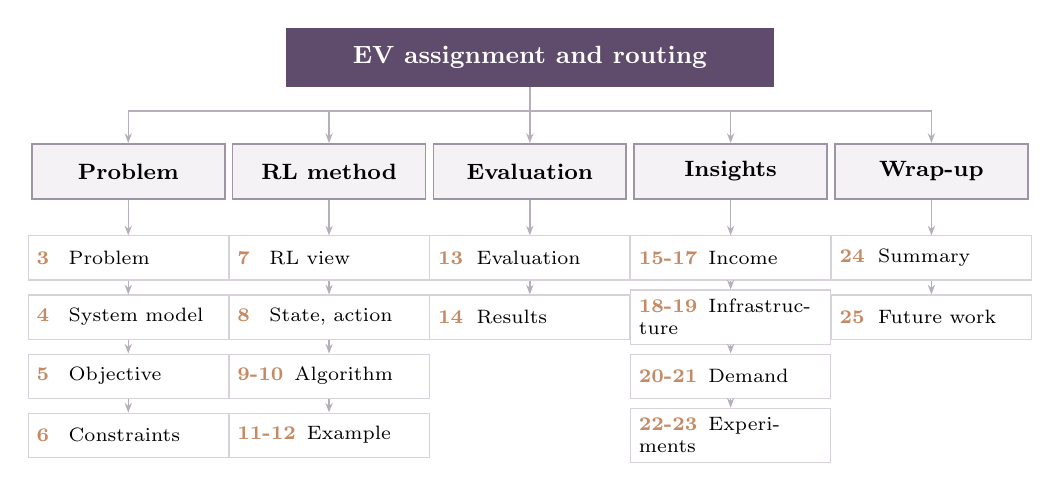
\begin{tikzpicture}[
 root/.style={fill=accP,text=white,minimum width=6.2cm,minimum height=.75cm,font=\small\bfseries},
 branch/.style={draw=accP!60,line width=.6pt,fill=accP!7,minimum width=2.45cm,minimum height=.7cm,font=\footnotesize\bfseries,align=center},
 leaf/.style={draw=accP!25,line width=.4pt,fill=white,text width=2.33cm,minimum height=.56cm,font=\scriptsize,align=left,inner xsep=3pt},
 arr/.style={-{Stealth[length=3.5pt]},accP!45,line width=.5pt}]
\node[root] (r) at (6.4,0) {EV assignment and routing};
\foreach \x/\n/\t in {1.3/b1/{Problem},3.85/b2/{RL method},6.4/b3/{Evaluation},8.95/b4/{Insights},11.5/b5/{Wrap-up}}{
  \node[branch] (\n) at (\x,-1.45) {\t};
  \draw[arr] (r.south) -- ++(0,-.3) -| (\n.north);
}
\node[leaf] (a1) at (1.3,-2.55) {\textcolor{accA}{\bfseries 3}\;\; Problem};
\node[leaf] (a2) at (1.3,-3.3)  {\textcolor{accA}{\bfseries 4}\;\; System model};
\node[leaf] (a3) at (1.3,-4.05) {\textcolor{accA}{\bfseries 5}\;\; Objective};
\node[leaf] (a4) at (1.3,-4.8)  {\textcolor{accA}{\bfseries 6}\;\; Constraints};
\node[leaf] (c1) at (3.85,-2.55) {\textcolor{accA}{\bfseries 7}\;\; RL view};
\node[leaf] (c2) at (3.85,-3.3)  {\textcolor{accA}{\bfseries 8}\;\; State, action};
\node[leaf] (c3) at (3.85,-4.05) {\textcolor{accA}{\bfseries 9-10}\, Algorithm};
\node[leaf] (c4) at (3.85,-4.8)  {\textcolor{accA}{\bfseries 11-12}\, Example};
\node[leaf] (d1) at (6.4,-2.55) {\textcolor{accA}{\bfseries 13}\; Evaluation};
\node[leaf] (d2) at (6.4,-3.3)  {\textcolor{accA}{\bfseries 14}\; Results};
\node[leaf] (e1) at (8.95,-2.55) {\textcolor{accA}{\bfseries 15-17}\, Income};
\node[leaf] (e2) at (8.95,-3.3)  {\textcolor{accA}{\bfseries 18-19}\, Infrastructure};
\node[leaf] (e3) at (8.95,-4.05) {\textcolor{accA}{\bfseries 20-21}\, Demand};
\node[leaf] (e4) at (8.95,-4.8)  {\textcolor{accA}{\bfseries 22-23}\, Experiments};
\node[leaf] (f1) at (11.5,-2.55) {\textcolor{accA}{\bfseries 24}\; Summary};
\node[leaf] (f2) at (11.5,-3.3)  {\textcolor{accA}{\bfseries 25}\; Future work};
\foreach \a/\b in {b1/a1,a1/a2,a2/a3,a3/a4,b2/c1,c1/c2,c2/c3,c3/c4,b3/d1,d1/d2,b4/e1,e1/e2,e2/e3,e3/e4,b5/f1,f1/f2}{\draw[arr] (\a) -- (\b);}
\end{tikzpicture}
\end{frame}

% ======================================================================= 3 problem
\begin{frame}{Problem}
\begin{itemize}
  \item A charging operator receives EV charging requests over a period $[0,T]$.
  \item Each request goes to a \textbf{station gun} (the EV drives there) or a \textbf{mobile van} (the van comes to the EV).
  \item The operator also routes the vans from and back to a depot.
  \item \textbf{Goal}: minimise operator cost + cost perceived by customers.
  \item Customers differ: \textbf{personal} or \textbf{commercial} (taxi), and by income $\theta\in[0,1]$.
  \item \textbf{Methods}: an exact MILP as benchmark; a reinforcement-learning policy for speed.
\end{itemize}
\end{frame}

% ======================================================================= 4 system model
\begin{frame}{System model}
\begin{columns}[T]
\column{.5\textwidth}
\centering
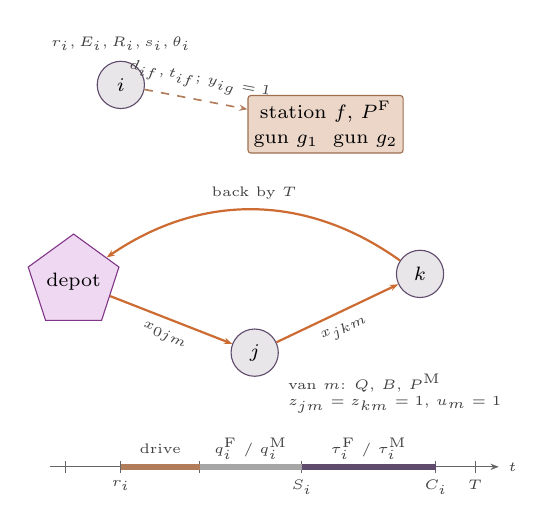
\begin{tikzpicture}[font=\scriptsize,
  ev/.style={circle,draw=accP,fill=cEV,inner sep=1pt,minimum size=6mm},
  st/.style={rectangle,rounded corners=1pt,draw=accA!80!black,fill=cFCS,inner sep=2pt,align=center},
  dp/.style={regular polygon,regular polygon sides=5,draw=gradPurple!70!black,fill=cDepot,minimum size=8mm,inner sep=0pt},
  drv/.style={-{Stealth[length=3pt]},accA!90!black,dashed,line width=.6pt},
  vn/.style={-{Stealth[length=3pt]},gradOrange!85!black,line width=.8pt},
  lab/.style={font=\tiny,text=black!75}]
\node[dp] (d) at (0,0) {depot};
\node[st] (f) at (3.2,2.0) {station $f$, $P^{\mathrm F}$\\[1pt] gun $g_1$ \ gun $g_2$};
\node[ev] (i) at (0.6,2.5) {$i$};
\node[lab,anchor=south] at (i.north) {$r_i,E_i,R_i,s_i,\theta_i$};
\node[ev] (j) at (2.3,-0.9) {$j$};
\node[ev] (k) at (4.4,0.1) {$k$};
\draw[drv] (i) -- node[lab,above,sloped]{$d_{if},t_{if}$; $y_{ig}=1$} (f);
\draw[vn] (d) -- node[lab,below,sloped]{$x_{0jm}$} (j);
\draw[vn] (j) -- node[lab,below,sloped]{$x_{jkm}$} (k);
\draw[vn] (k) to[bend right=35] node[lab,above,sloped]{back by $T$} (d);
\node[lab,align=left,anchor=north west] at (2.6,-1.05) {van $m$: $Q$, $B$, $P^{\mathrm M}$\\ $z_{jm}=z_{km}=1$, $u_m=1$};
% timeline
\draw[-{Stealth[length=3pt]},black!60] (-0.3,-2.35) -- (5.4,-2.35) node[lab,right]{$t$};
\foreach \x/\l in {-0.1/0, 0.6/r_i, 1.6/{\ }, 2.9/S_i, 4.6/C_i, 5.1/T}{\draw[black!60] (\x,-2.43) -- (\x,-2.27);}
\node[lab,below] at (0.6,-2.4) {$r_i$};
\node[lab,below] at (2.9,-2.4) {$S_i$};
\node[lab,below] at (4.6,-2.4) {$C_i$};
\node[lab,below] at (5.1,-2.4) {$T$};
\draw[accA!90!black,line width=2pt] (0.6,-2.35) -- (1.6,-2.35);
\draw[black!35,line width=2pt] (1.6,-2.35) -- (2.9,-2.35);
\draw[accP,line width=2pt] (2.9,-2.35) -- (4.6,-2.35);
\node[lab] at (1.1,-2.12) {drive};
\node[lab] at (2.25,-2.12) {$q^{\mathrm F}_i$ / $q^{\mathrm M}_i$};
\node[lab] at (3.75,-2.12) {$\tau^{\mathrm F}_i$ / $\tau^{\mathrm M}_i$};
\end{tikzpicture}
\column{.47\textwidth}
\scriptsize
\begin{tabular}{@{}ll@{}}
\toprule
symbol & meaning\\
\midrule
$r_i,E_i,R_i$ & request time, energy (kWh), range (km)\\
$s_i,\theta_i$ & segment, income index\\
$f,g$; $P^{\mathrm F}$ & station, gun; 22\,kW\\
$m$; $Q,B,P^{\mathrm M}$ & van; 6 EVs, 150\,kWh, 30\,kW\\
$y_{ig}$, $z_{im}$ & EV $i$ on gun $g$ / van $m$\\
$x_{ijm}$, $u_m$ & van $m$ drives $i\to j$; van used\\
$S_i$, $C_i$ & start, finish of charging\\
$q^{\mathrm F}_i$, $q^{\mathrm M}_i$ & queue at station, wait for van\\
$\tau^{\mathrm F}_i,\tau^{\mathrm M}_i$ & charging time $=60E_i/P$\\
$T$ & horizon: all done by $T$\\
\bottomrule
\end{tabular}
\end{columns}
\end{frame}

% ======================================================================= 5 objective
\begin{frame}{Optimisation problem: objective}
\scriptsize
\vspace{-.5ex}
$\min Z=Z_1+\dots+Z_6$, \ with $\mu_i=\mu^{s_i}(\theta_i)$, $c^a_i=c^{a,s_i}(\theta_i)$ linear in $\theta_i$.\\[.6ex]
\renewcommand{\arraystretch}{1.0}
\begin{tabular}{@{}p{.5\textwidth}@{\hspace{2mm}}p{.47\textwidth}@{}}
$Z_1=\sum_i \mu_i\,c^{\mathrm{EV}}\sum_{f}d_{if}Y_{if}$ &
\begin{termbox}\textbf{EV driving}, perceived: km to the station $\times$ Rs/km; $Y_{if}$ = EV $i$ uses station $f$.\end{termbox}\\[-2.5ex]
$Z_2=c^{\mathrm M}\sum_m\sum_{(i,j)}d_{ij}x_{ijm}$ &
\begin{termbox}[accA]\textbf{Van km} (operator); $x_{ijm}$ = van route arcs.\end{termbox}\\[-2.5ex]
$Z_3=\sum_m c^{\mathrm F}_m u_m$ &
\begin{termbox}[accA]\textbf{Van dispatch} (operator): fixed cost per van used, $u_m$.\end{termbox}\\[-2.5ex]
$Z_4=\pi^{\mathrm F}\sum_i E_iy_i+\pi^{\mathrm M}\sum_i\frac{E_i}{\eta}z_i$ &
\begin{termbox}[accA]\textbf{Energy} (operator); van transfer loses $1-\eta$; $y_i,z_i$ = station / van.\end{termbox}\\[-2.5ex]
$Z_5=\sum_i \mu_i E_i\big(p^{\mathrm F}y_i+p^{\mathrm M}z_i\big)$ &
\begin{termbox}\textbf{Tariff}, perceived: price paid $\times$ money sensitivity $\mu_i$.\end{termbox}\\[-2.5ex]
$\begin{aligned}Z_6=\sum_i\Big(&c^{\mathrm D}_i\textstyle\sum_f t_{if}Y_{if}+c^{\mathrm Q}_iq^{\mathrm F}_i\\[-2pt]&+c^{\mathrm C}_i\tau^{\mathrm F}_iy_i+c^{\mathrm V}_i(q^{\mathrm M}_i+\tau^{\mathrm M}_iz_i)\Big)\end{aligned}$ &
\begin{termbox}\textbf{Time}, perceived: driving, queueing, charging, van wait + charging, each at the customer's value of time; $q^{\mathrm F}_i,q^{\mathrm M}_i$ waits.\end{termbox}\\
\end{tabular}

\vspace{-.5ex}
\textcolor{accA}{\rule{6pt}{6pt}} operator cost $Z_2{+}Z_3{+}Z_4$ \quad \textcolor{accP!70}{\rule{6pt}{6pt}} customer cost $Z_1{+}Z_5{+}Z_6$
\end{frame}

% ======================================================================= 6 constraints
\begin{frame}{Constraints}
\scriptsize
\begin{columns}[T]
\column{.5\textwidth}
\textbf{Assignment}
\[ \textstyle\sum_{g\in G_i}y_{ig}+\sum_{m}z_{im}=1 \]
\textbf{Station sequencing and queue}
\[ \begin{aligned}
&S_i\ge r_i+\textstyle\sum_f t_{if}Y_{if},\quad q^{\mathrm F}_i+q^{\mathrm M}_i=S_i-r_i-\sum_f t_{if}Y_{if}\\
&q^{\mathrm F}_i\le W_iy_i,\qquad q^{\mathrm M}_i\le T z_i\\
&S_j\ge S_i+\tau^{\mathrm F}_i-M^{\mathrm F}_i(3-y_{ig}-y_{jg}-o_{ij})\ \ (\text{and reverse})
\end{aligned} \]
\textbf{Van routing}
\[ \textstyle\sum_j x_{0jm}=u_m=\sum_i x_{i,n+1,m},\qquad \sum_i x_{ijm}=z_{jm}=\sum_k x_{jkm} \]
\column{.48\textwidth}
\textbf{Van capacity and battery}
\[ \textstyle\sum_i z_{im}\le Q\,u_m,\qquad \sum_i\frac{E_i}{\eta}z_{im}+\beta\sum_{(i,j)}d_{ij}x_{ijm}\le B\,u_m \]
\textbf{Timing and horizon}
\[ \begin{aligned}
&S_j\ge t_{0j}x_{0jm},\quad S_j\ge S_i+\tau^{\mathrm M}_i+t_{ij}-M^{\mathrm M}_{ij}(1-x_{ijm})\\
&S_i+\tau^{\mathrm M}_i+t_{i,0}\le T\ \text{ if } i \text{ is a van's last stop}\\
&S_i\ge r_i,\qquad C_i\le T
\end{aligned} \]
\textbf{Symmetry and domains}: twin guns used in order; vans used in order; binaries $y,z,x,u,o$; $S,q\ge0$.
\end{columns}
\end{frame}

% ======================================================================= 7 RL view
\begin{frame}{RL representation}
\begin{columns}[T]
\column{.6\textwidth}
\centering
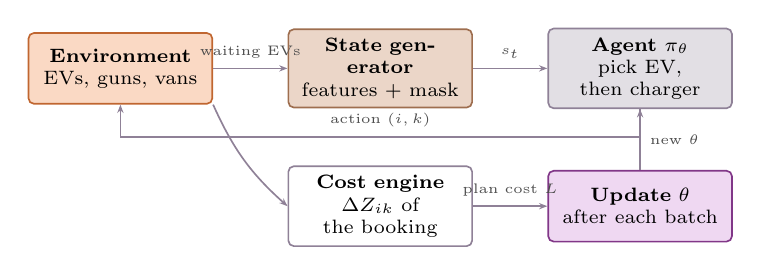
\begin{tikzpicture}[font=\scriptsize,
  bx/.style={draw=accP!70,rounded corners=2pt,align=center,text width=2.1cm,minimum height=.9cm,line width=.6pt,fill=white},
  env/.style={bx,fill=cVan,draw=gradOrange!80!black},
  gen/.style={bx,fill=cFCS,draw=accA!80!black},
  ag/.style={bx,fill=cNet},
  up/.style={bx,fill=cDepot,draw=gradPurple!70!black},
  a/.style={-{Stealth[length=3pt]},accP!70,line width=.6pt},
  lab/.style={font=\tiny,text=black!70}]
\node[env] (e) at (0,0) {\textbf{Environment}\\ EVs, guns, vans};
\node[gen] (s) at (3.3,0) {\textbf{State generator}\\ features + mask};
\node[ag] (p) at (6.6,0) {\textbf{Agent} $\pi_\theta$\\ pick EV, then charger};
\node[bx] (c) at (3.3,-1.75) {\textbf{Cost engine}\\ $\Delta Z_{ik}$ of the booking};
\node[up] (u) at (6.6,-1.75) {\textbf{Update} $\theta$\\ after each batch};
\draw[a] (e) -- node[lab,above]{waiting EVs} (s);
\draw[a] (s) -- node[lab,above]{$s_t$} (p);
\draw[a] (p.south) -- ++(0,-0.35) -| node[lab,above,pos=0.25]{action $(i,k)$} (e.south);
\draw[a] (e.south east) to[bend right=12] (c.west);
\draw[a] (c) -- node[lab,above]{plan cost $L$} (u);
\draw[a] (u) -- node[lab,right]{new $\theta$} (p);
\end{tikzpicture}

\vspace{1ex}
\scriptsize One episode = one complete plan; one step = one booking.
\column{.37\textwidth}
\small
\textbf{Mask}: a pair $(i,k)$ is feasible if
\begin{itemize}
  \item station within range $R_i$
  \item queue $\le W_i$
  \item charging done by $T$
  \item van: free seat, battery for $i$ and the return, back by $T$
\end{itemize}
\textbf{Symmetry pruning}: of equally free twin guns and of unused vans, only the first is offered.
\end{columns}
\end{frame}

% ======================================================================= 8 state, action, reward
\begin{frame}{State, action, reward}
\begin{columns}[T]
\column{.5\textwidth}
\scriptsize
\textbf{State}: static features (EV 19, station 4, depot 4) + dynamic features (global 4, EV 7, charger 6, pair 6), e.g.\ gun free times, van position, battery, seats, cheapest option, regret.

\textbf{Action}: pair (EV $i$, charger $k$); $i$ joins the end of $k$'s queue or route.

\textbf{Reward} $=-\Delta Z_{ik}$:
\[ \begin{aligned}
\Delta Z^{\text{gun}}&=\mu_i(c^{\mathrm{EV}}d_{if}+p^{\mathrm F}E_i)+\pi^{\mathrm F}E_i+c^{\mathrm D}_it_{if}+c^{\mathrm C}_i\tau^{\mathrm F}_i+c^{\mathrm Q}_iw_{ik}\\
\Delta Z^{\text{van}}&=\mu_ip^{\mathrm M}E_i+\tfrac{\pi^{\mathrm M}E_i}{\eta}+c^{\mathrm V}_i(\tau^{\mathrm M}_i+w_{im})\\[-2pt]
&\quad+c^{\mathrm M}(d_{p,i}+d_{i,0}-d_{p,0})+c^{\mathrm F}\,[\text{van unused}]
\end{aligned} \]
\textbf{Plan cost} \ $L=Z+10\,\sigma\cdot\text{dropped EVs}$
\column{.47\textwidth}
\scriptsize
\textbf{Normalisation}
\begin{itemize}
  \item times $\div T$, costs $\div\sigma$ (mean cheapest first option), battery $\div B$, seats $\div Q$: one network for any city, horizon and size.
  \item advantage $\div$ mean plan cost: small and large instances weigh equally.
\end{itemize}
\textbf{Rules}
\begin{itemize}
  \item Start as early as possible: $S=\max(\text{arrival},\text{gun or van free})$; a busy charger means the EV waits in its queue or route.
  \item An EV with no feasible charger is dropped: queues only grow and batteries only shrink, so it never becomes feasible.
  \item Warm-up teacher orders EVs: stranded, then $r_i$, ties by larger $c^{\mathrm Q}_i$.
\end{itemize}
\end{columns}
\end{frame}

% ======================================================================= 9 algorithm
\begin{frame}{Training algorithm}
\begin{columns}[T]
\column{.56\textwidth}
\begin{algorithm}[H]
\caption{RL Training}
\For{epoch $=1$ \KwTo 500}{
  \For{batch $=1$ \KwTo 50}{
    Generate 32 random instances (same $n$)\;
    \eIf{first 500 batches (warm-up)}{
      copy the greedy rule: loss $=-\frac1n\log\pi_\theta(\text{rule plan})$\;
    }{
      8 sampled episodes per instance, costs $L_j$\;
      loss $=$ mean $A_j\log\pi_\theta(\text{plan}_j)$, $A_j=(L_j-\bar L)/\bar L$\;
    }
    Adam step on $\theta$ (gradient norm $\le 1$)\;
  }
  Validate against the greedy rule; keep the best $\theta$\;
}
\end{algorithm}
\column{.4\textwidth}
\small
\begin{itemize}
  \item \textbf{REINFORCE}\footnote{R.\,J.~Williams, Simple statistical gradient-following algorithms for connectionist RL, \emph{Machine Learning} 8, 1992.}: whole-plan cost, no per-step learning.
  \item \textbf{Shared baseline}\footnote{Y.~Kwon et al., POMO: policy optimization with multiple optima for RL, NeurIPS 2020.} $\bar L$: mean of 8 plans of the same instance; no critic, no replay buffer.
  \item \textbf{Warm-up}: imitate the greedy rule first.
  \item Stop: 10 epochs without gain after epoch 200.
\end{itemize}
\end{columns}
\end{frame}

% ======================================================================= 10 network
\begin{frame}{Policy network: encoder and decoder}
\centering
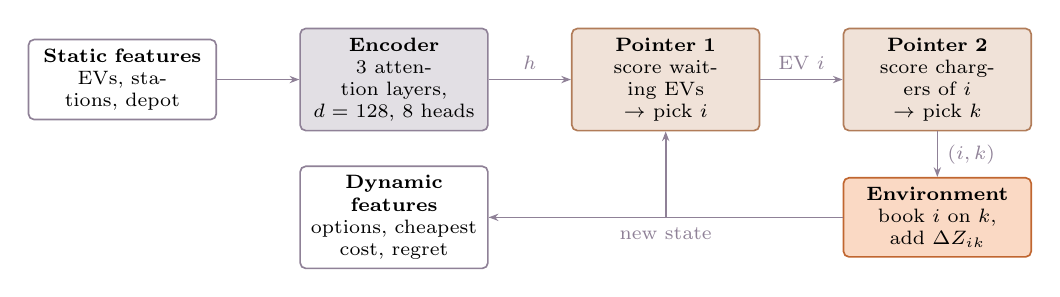
\begin{tikzpicture}[font=\scriptsize,
  bx/.style={draw=accP!70,fill=white,rounded corners=2pt,align=center,minimum height=.95cm,text width=2.15cm,line width=.6pt},
  enc/.style={bx,fill=cNet},
  ptr/.style={bx,fill=cPtr,draw=accA!90!black},
  envb/.style={bx,fill=cVan,draw=gradOrange!80!black},
  a/.style={-{Stealth[length=3.5pt]},accP!70,line width=.6pt}]
\node[bx] (in) at (0,0) {\textbf{Static features}\\ EVs, stations, depot};
\node[enc] (enc) at (3.45,0) {\textbf{Encoder}\\ 3 attention layers,\\ $d=128$, 8 heads};
\node[bx] (dyn) at (3.45,-1.75) {\textbf{Dynamic features}\\ options, cheapest cost, regret};
\node[ptr] (p1) at (6.9,0) {\textbf{Pointer 1}\\ score waiting EVs\\ $\to$ pick $i$};
\node[ptr] (p2) at (10.35,0) {\textbf{Pointer 2}\\ score chargers of $i$\\ $\to$ pick $k$};
\node[envb] (env) at (10.35,-1.75) {\textbf{Environment}\\ book $i$ on $k$, add $\Delta Z_{ik}$};
\draw[a] (in) -- (enc);
\draw[a] (enc) -- node[above]{$h$} (p1);
\draw[a] (p1) -- node[above]{EV $i$} (p2);
\draw[a] (dyn) -| (p1);
\draw[a] (p2) -- node[right]{$(i,k)$} (env);
\draw[a] (env) -- node[below]{new state} (dyn);
\end{tikzpicture}

\vspace{1.2ex}
\raggedright
\small
\begin{itemize}
  \item \textbf{Embedding} $h_i$: a vector per EV that, through attention\footnote{A.~Vaswani et al., Attention is all you need, NeurIPS 2017.}, mixes its own data with nearby stations, other EVs and their costs.
  \item \textbf{Decoder}\footnote{W.~Kool, H.~van Hoof, M.~Welling, Attention, learn to solve routing problems!, ICLR 2019.}: points to an EV, then to a charger; infeasible choices masked; \Params{} parameters.
\end{itemize}
\end{frame}

% ======================================================================= 11 example t = 0
\begin{frame}{Representative example: step $t=0$}
\centering
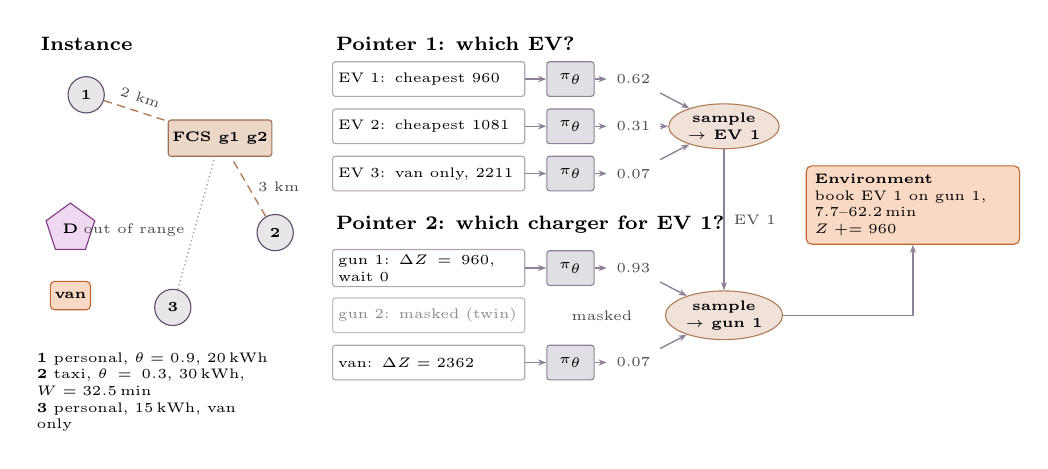
\begin{tikzpicture}[font=\scriptsize,
  ev/.style={circle,draw=accP,fill=cEV,inner sep=0.6pt,minimum size=4.6mm,font=\tiny\bfseries},
  st/.style={rectangle,rounded corners=1pt,draw=accA!80!black,fill=cFCS,minimum height=4.6mm,inner sep=1.5pt,font=\tiny\bfseries},
  dp/.style={regular polygon,regular polygon sides=5,draw=gradPurple!70!black,fill=cDepot,minimum size=6.5mm,inner sep=0pt,font=\tiny\bfseries},
  van/.style={rectangle,rounded corners=1.5pt,draw=gradOrange!80!black,fill=cVan,minimum height=3.6mm,inner sep=1.5pt,font=\tiny\bfseries},
  opt/.style={accA!90!black,densely dashed,line width=.5pt},
  bad/.style={black!35,densely dotted,line width=.5pt},
  inp/.style={draw=accP!50,fill=white,rounded corners=1pt,minimum height=4.4mm,inner sep=2pt,align=left,text width=2.3cm,font=\tiny},
  nn/.style={draw=accP!70,fill=cNet,rounded corners=1pt,minimum width=6mm,minimum height=4.4mm,inner sep=0pt,font=\tiny\bfseries},
  pick/.style={ellipse,draw=accA!90!black,fill=cPtr,inner sep=1pt,font=\tiny\bfseries,align=center},
  envb/.style={draw=gradOrange!80!black,fill=cVan,rounded corners=2pt,align=left,text width=2.5cm,inner sep=3pt,font=\tiny},
  a/.style={-{Stealth[length=3pt]},accP!70,line width=.5pt},
  lab/.style={font=\tiny,text=black!70}]
\node[font=\scriptsize\bfseries,anchor=west] at (-0.2,0.45) {Instance};
\node[dp] (d) at (0.3,-1.9) {D};
\node[st] (s) at (2.2,-0.75) {FCS g1 g2};
\node[van] (v) at (0.3,-2.75) {van};
\node[ev] (e1) at (0.5,-0.2) {1};
\node[ev] (e2) at (2.9,-1.95) {2};
\node[ev] (e3) at (1.6,-2.9) {3};
\draw[opt] (e1) -- node[lab,above,sloped]{2 km} (s);
\draw[opt] (e2) -- node[lab,right]{3 km} (s);
\draw[bad] (e3) -- node[lab,left,pos=.45]{out of range} (s);
\node[align=left,anchor=north west,font=\tiny,text width=3.0cm] at (-0.25,-3.35)
 {\textbf{1} personal, $\theta=0.9$, 20\,kWh\\ \textbf{2} taxi, $\theta=0.3$, 30\,kWh, $W=\ToyWTwo$\,min\\ \textbf{3} personal, 15\,kWh, van only};
\node[font=\scriptsize\bfseries,anchor=west] at (3.55,0.45) {Pointer 1: which EV?};
\foreach \k/\y/\t/\p in {1/0/{EV 1: cheapest \ToyGunOne}/0.62, 2/-0.6/{EV 2: cheapest \ToyGunTwo}/0.31, 3/-1.2/{EV 3: van only, \ToyVanThree}/0.07}{
  \node[inp] (i\k) at (4.85,\y) {\t};
  \node[nn] (n\k) at (6.65,\y) {$\pi_\theta$};
  \node[lab] (p\k) at (7.45,\y) {\p};
  \draw[a] (i\k) -- (n\k); \draw[a] (n\k) -- (p\k);
}
\node[pick] (k1) at (8.6,-0.6) {sample\\ $\to$ EV 1};
\foreach \k in {1,2,3}{\draw[a] (p\k) -- (k1);}
\node[font=\scriptsize\bfseries,anchor=west] at (3.55,-1.85) {Pointer 2: which charger for EV 1?};
\node[inp] (j1) at (4.85,-2.4) {gun 1: $\Delta Z=\ToyGunOne$, wait 0};
\node[inp,draw=black!25,text=black!45] (j2) at (4.85,-3.0) {gun 2: masked (twin)};
\node[inp] (j3) at (4.85,-3.6) {van: $\Delta Z=\ToyVanOne$};
\foreach \k/\y/\p in {1/-2.4/0.93, 3/-3.6/0.07}{
  \node[nn] (m\k) at (6.65,\y) {$\pi_\theta$};
  \node[lab] (q\k) at (7.45,\y) {\p};
  \draw[a] (j\k) -- (m\k); \draw[a] (m\k) -- (q\k);
}
\node[lab] at (7.05,-3.0) {masked};
\node[pick] (k2) at (8.6,-3.0) {sample\\ $\to$ gun 1};
\draw[a] (q1) -- (k2); \draw[a] (q3) -- (k2);
\draw[a] (k1) -- node[lab,right]{EV 1} (k2);
\node[envb] (env) at (11.0,-1.6) {\textbf{Environment}\\ book EV 1 on gun 1,\\ \ToyStartOne--\ToyEndOne\,min\\ $Z \mathrel{+}= \ToyGunOne$};
\draw[a] (k2.east) -| (env.south);
\end{tikzpicture}

\vspace{-.2ex}
{\tiny $\Delta Z$ in Rs, exact for this toy instance (van includes \ToyDispatch{} dispatch); probabilities illustrative.}
\end{frame}

% ======================================================================= 12 example t = k
\begin{frame}{Representative example: later steps}
\centering
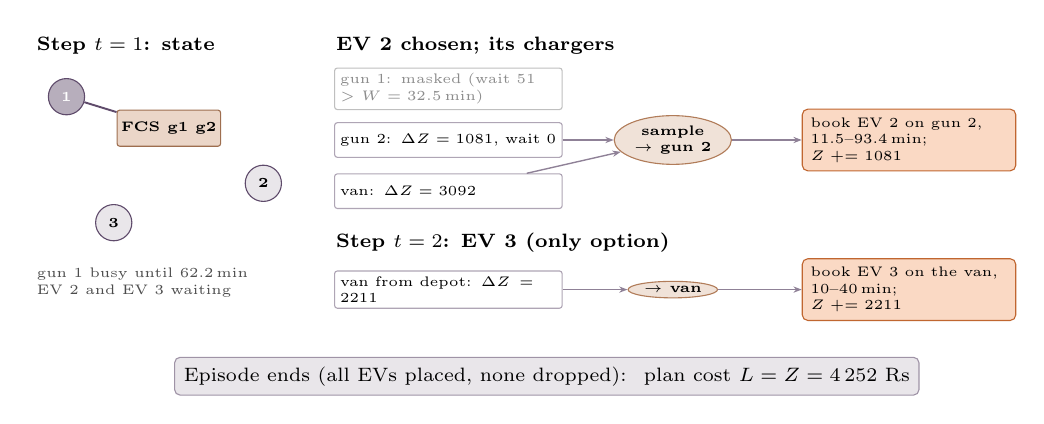
\begin{tikzpicture}[font=\scriptsize,
  ev/.style={circle,draw=accP,fill=cEV,inner sep=0.6pt,minimum size=4.6mm,font=\tiny\bfseries},
  evd/.style={ev,fill=accP!45,text=white},
  st/.style={rectangle,rounded corners=1pt,draw=accA!80!black,fill=cFCS,minimum height=4.6mm,inner sep=1.5pt,font=\tiny\bfseries},
  dp/.style={regular polygon,regular polygon sides=5,draw=gradPurple!70!black,fill=cDepot,minimum size=6.5mm,inner sep=0pt,font=\tiny\bfseries},
  van/.style={rectangle,rounded corners=1.5pt,draw=gradOrange!80!black,fill=cVan,minimum height=3.6mm,inner sep=1.5pt,font=\tiny\bfseries},
  inp/.style={draw=accP!50,fill=white,rounded corners=1pt,minimum height=4.4mm,inner sep=2pt,align=left,text width=2.75cm,font=\tiny},
  pick/.style={ellipse,draw=accA!90!black,fill=cPtr,inner sep=1pt,font=\tiny\bfseries,align=center},
  envb/.style={draw=gradOrange!80!black,fill=cVan,rounded corners=2pt,align=left,text width=2.5cm,inner sep=3pt,font=\tiny},
  a/.style={-{Stealth[length=3pt]},accP!70,line width=.5pt},
  lab/.style={font=\tiny,text=black!70}]
% step t = 1
\node[font=\scriptsize\bfseries,anchor=west] at (-0.2,0.45) {Step $t=1$: state};
\node[st] (s) at (1.6,-0.6) {FCS g1 g2};
\node[evd] (f1) at (0.3,-0.2) {1};
\node[ev] (f2) at (2.8,-1.3) {2};
\node[ev] (f3) at (0.9,-1.8) {3};
\draw[accP,line width=.7pt] (f1) -- (s);
\node[lab,align=left,anchor=north west] at (-0.2,-2.25) {gun 1 busy until \ToyEndOne\,min\\ EV 2 and EV 3 waiting};
\node[font=\scriptsize\bfseries,anchor=west] at (3.6,0.45) {EV 2 chosen; its chargers};
\node[inp,draw=black!25,text=black!45] (g1) at (5.15,-0.1) {gun 1: masked (wait \ToyWaitTwo{} $>$ $W=\ToyWTwo$\,min)};
\node[inp] (g2) at (5.15,-0.75) {gun 2: $\Delta Z=\ToyGunTwo$, wait 0};
\node[inp] (gv) at (5.15,-1.4) {van: $\Delta Z=\ToyVanTwo$};
\node[pick] (k) at (8.0,-0.75) {sample\\ $\to$ gun 2};
\draw[a] (g2) -- (k); \draw[a] (gv) -- (k);
\node[envb] (e2) at (11.0,-0.75) {book EV 2 on gun 2,\\ \ToyStartTwo--\ToyEndTwo\,min;\\ $Z \mathrel{+}= \ToyGunTwo$};
\draw[a] (k) -- (e2);
% step t = 2
\node[font=\scriptsize\bfseries,anchor=west] at (3.6,-2.05) {Step $t=2$: EV 3 (only option)};
\node[inp] (g3) at (5.15,-2.65) {van from depot: $\Delta Z=\ToyVanThree$};
\node[pick] (k3) at (8.0,-2.65) {$\to$ van};
\draw[a] (g3) -- (k3);
\node[envb] (e3) at (11.0,-2.65) {book EV 3 on the van,\\ \ToyStartThree--\ToyEndThree\,min;\\ $Z \mathrel{+}= \ToyVanThree$};
\draw[a] (k3) -- (e3);
\node[draw=accP!60,fill=cEV,rounded corners=2pt,font=\scriptsize,align=center] at (6.4,-3.75)
 {Episode ends (all EVs placed, none dropped): \ plan cost $L=Z=\ToyTotal$ Rs};
\end{tikzpicture}

\vspace{-.2ex}
{\tiny $\Delta Z$ exact for the toy instance; the choices shown are one possible sample.}
\end{frame}

% ======================================================================= 13 evaluation
\begin{frame}{Evaluation}
\begin{columns}[T]
\column{.5\textwidth}
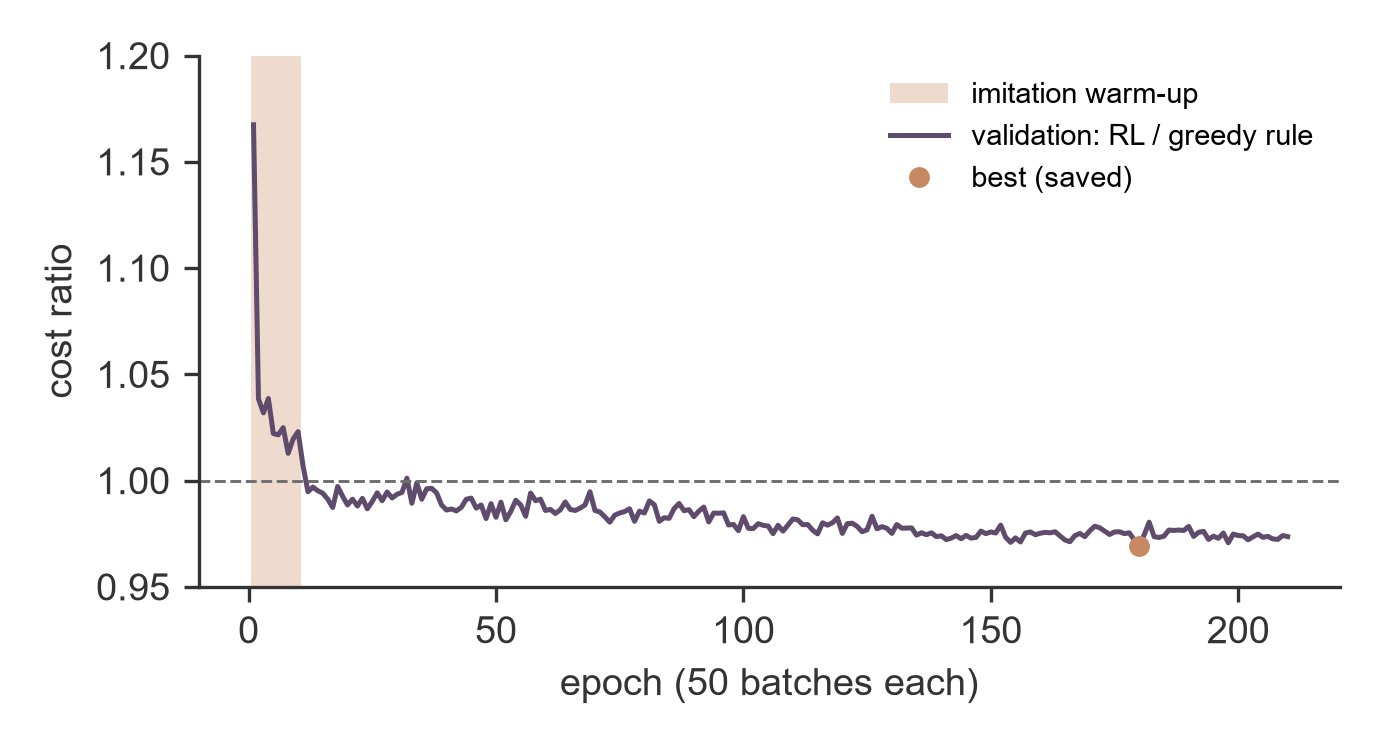
\includegraphics[width=\textwidth]{figures/training.png}

\vspace{.3ex}
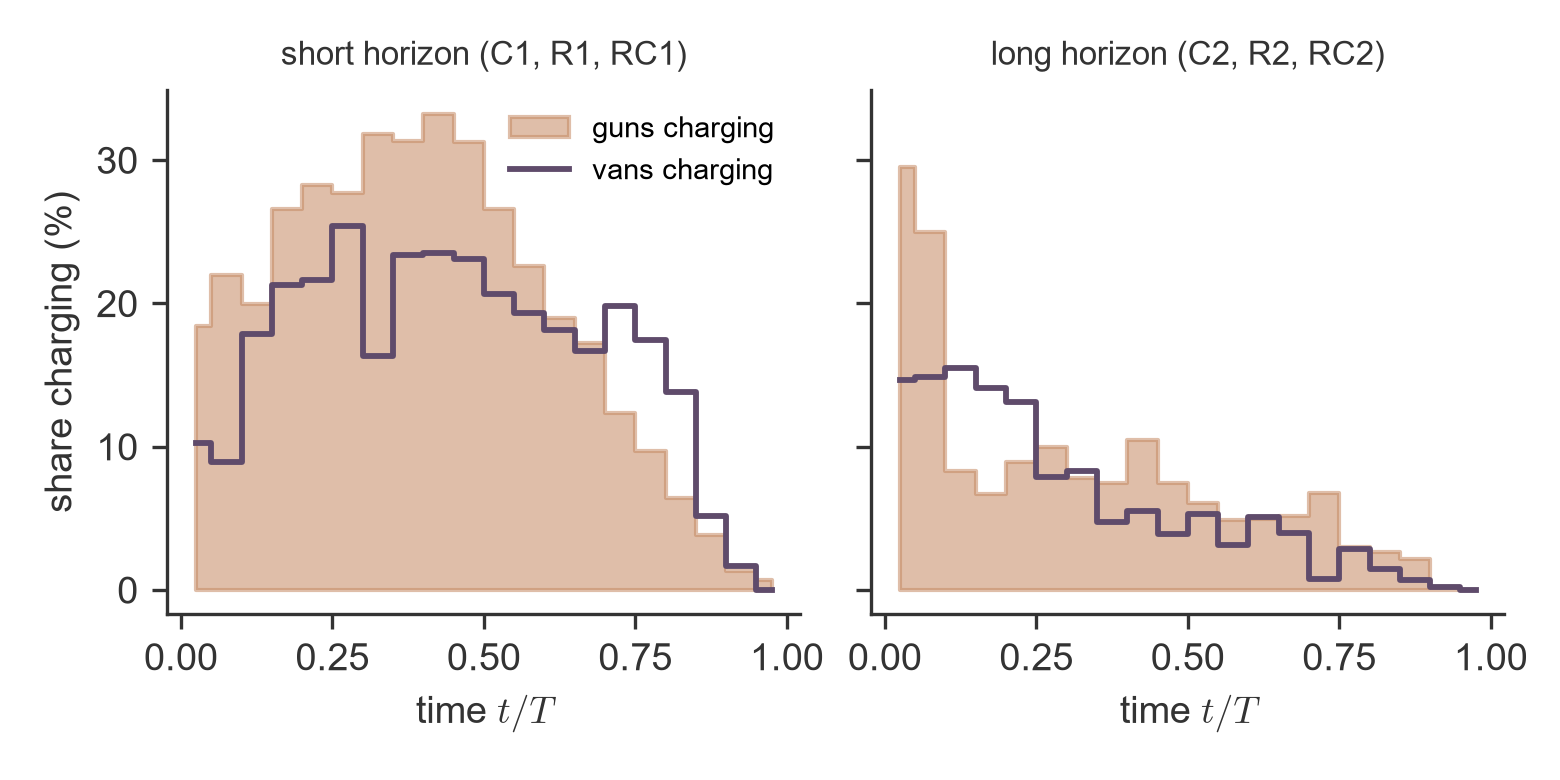
\includegraphics[width=\textwidth]{figures/busy.png}
\column{.47\textwidth}
\small
\textbf{Why this approach}
\begin{itemize}
  \item MILP\footnote{Gurobi Optimizer 13, Gurobi Optimization LLC.} is exact but hits the 300\,s limit from $n\approx40$.
  \item RL plans in a fraction of a second and works for any size.
\end{itemize}
\textbf{How quality is checked}
\begin{itemize}
  \item An independent checker re-tests every constraint and recomputes $Z$.
  \item Benchmarks: MILP (exact) and the greedy rule.
  \item Training: RL beats the greedy rule by \TrainBestGain\% on validation (best epoch \BestEpoch).
\end{itemize}
\scriptsize Bottom left: share of guns and vans charging over time (MILP).
\end{columns}
\end{frame}

% ======================================================================= 14 results
\begin{frame}{Results: MILP vs RL}
\begin{columns}[T]
\column{.55\textwidth}
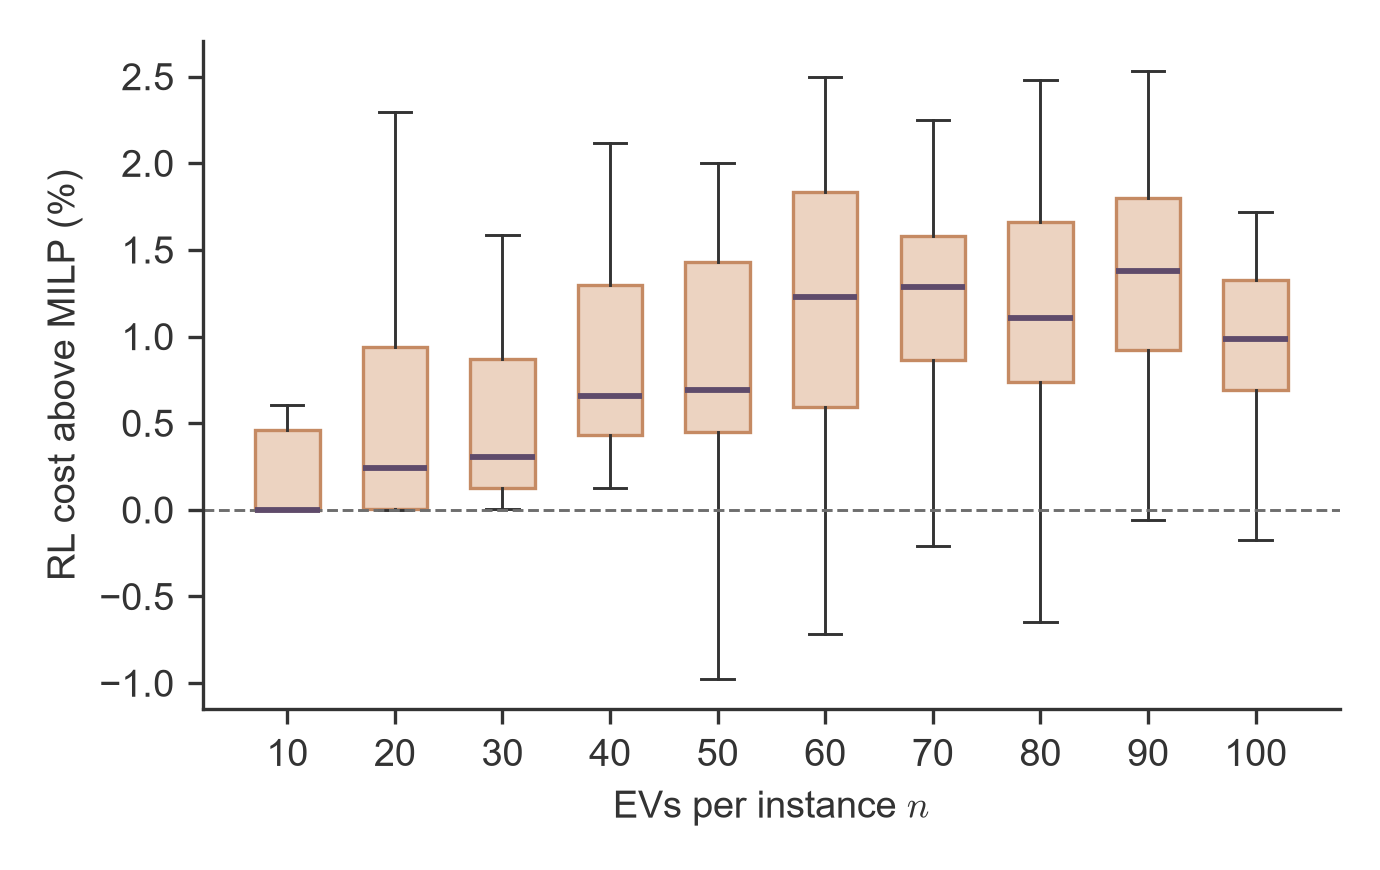
\includegraphics[width=\textwidth]{figures/gap.png}
\column{.42\textwidth}
\small
\begin{tabular}{lrr}
\toprule
 & MILP & RL\\
\midrule
valid plans (of 560) & \NValidM & \NValidR\\
optimal & \NOpt & --\\
cost above MILP & -- & \GapMean\%\\
time / instance & \TimeM\,s & \TimeR\,s\\
\bottomrule
\end{tabular}

\vspace{1ex}
\begin{itemize}
  \item RL is \Speed{}$\times$ faster; plans \RlOnly{} instances the MILP cannot.
  \item RL test: 8 map rotations $\times$ (1 greedy + 64 sampled) = 520 plans, best kept.
  \item MILP: 300\,s, 32 cores; data: Solomon instances\footnote{M.\,M.~Solomon, Algorithms for the vehicle routing and scheduling problems with time window constraints, \emph{Operations Research} 35(2), 1987.}.
\end{itemize}
\end{columns}
\end{frame}

% ======================================================================= 15 income and segment: MILP
\begin{frame}{Income and segment: who gets a van}
\begin{columns}[T]
\column{.55\textwidth}
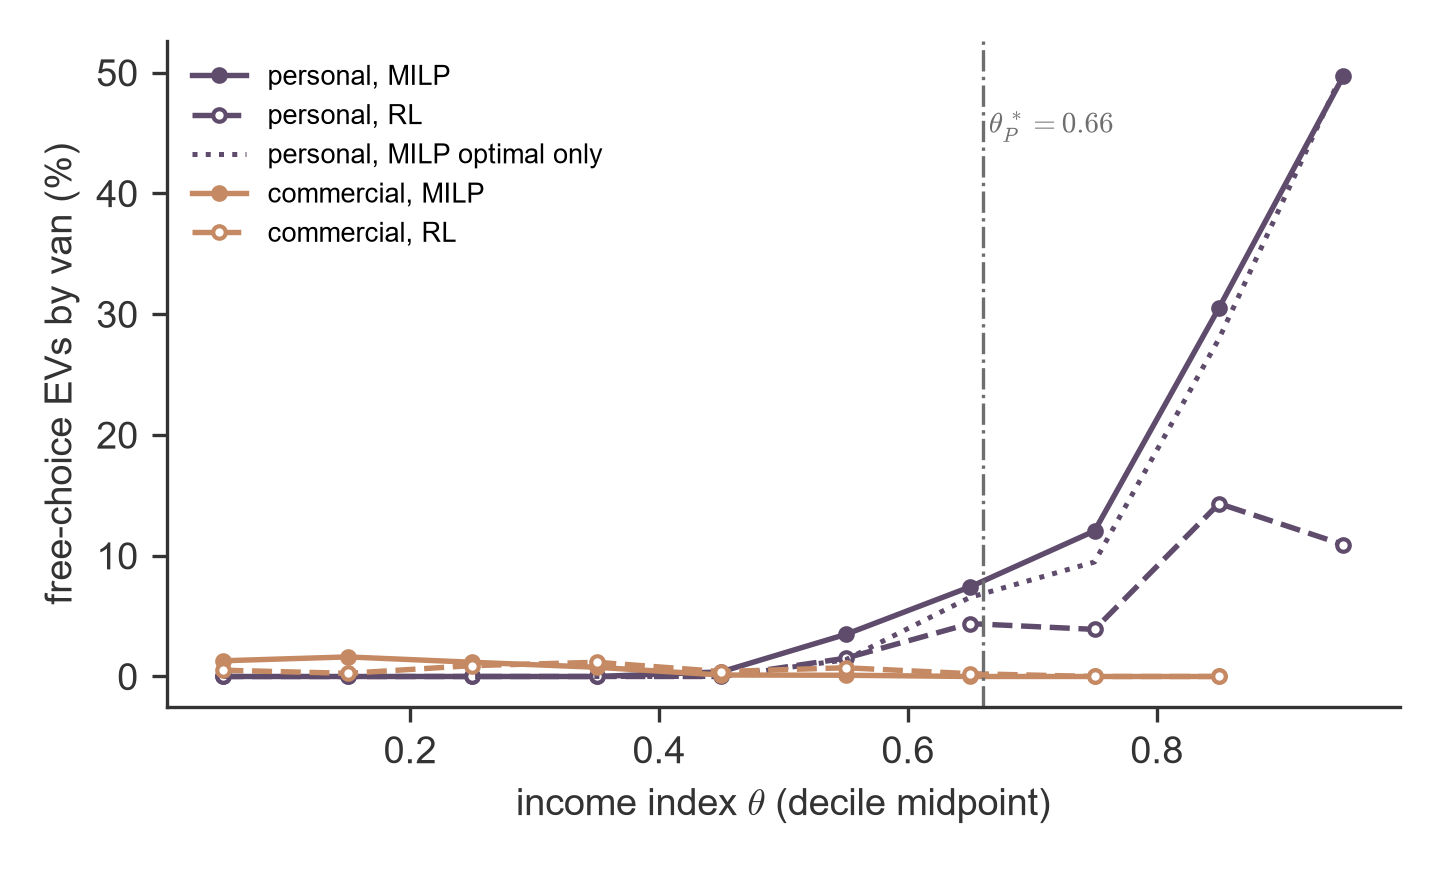
\includegraphics[width=\textwidth]{figures/van_decile.png}
\column{.42\textwidth}
\small
\begin{itemize}
  \item Personal: \VanPersonalMilp\% by van (MILP), \VanPersonalRl\% (RL).
  \item Optimal plans: none below $\theta=0.4$, \VanPersOptTop\% in the top decile.
  \item Theory: threshold $\theta^*_P=\ThetaStarP$; the data step is there.
  \item Taxis: \VanCommercialMilp\%; a van pays off only behind a $\ge$\QueueNeedCom{} min queue.
\end{itemize}
\end{columns}
\end{frame}

% ======================================================================= 16 income and segment: service
\begin{frame}{Income and segment: service}
\begin{columns}[T]
\column{.58\textwidth}
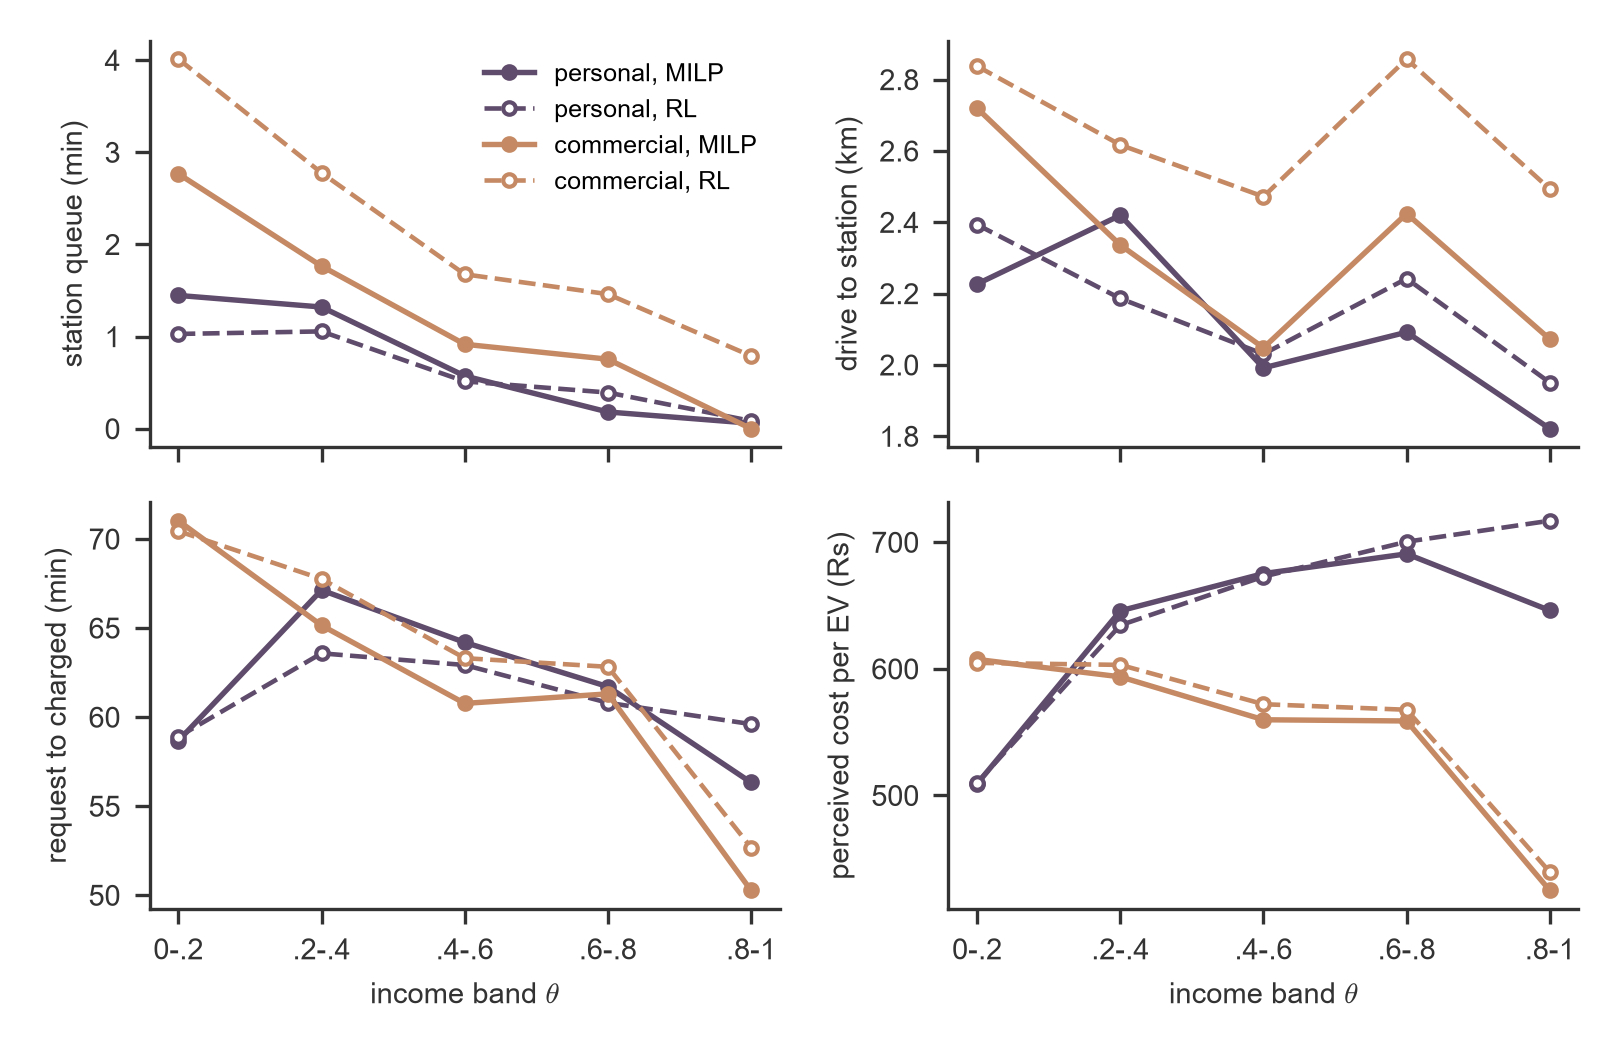
\includegraphics[width=\textwidth]{figures/seg_income.png}
\column{.39\textwidth}
\small
\begin{itemize}
  \item Poorer EVs queue longer and drive farther; taxis most.
  \item Rich personal owners: short queue, short drive, often a van.
  \item RL: same pattern, longer taxi queues.
\end{itemize}
\vspace{.5ex}
\scriptsize Station users; MILP solid, RL dashed.
\end{columns}
\end{frame}

% ======================================================================= 17 who queues, who pays
\begin{frame}{Income and segment: who queues, who pays}
\begin{columns}[T]
\column{.47\textwidth}
\scriptsize
\textbf{Station users vs queue minutes (\%)}\\[.5ex]
\setlength{\tabcolsep}{4pt}
\begin{tabular}{lrrrr}
\toprule
 & \multicolumn{2}{c}{MILP} & \multicolumn{2}{c}{RL}\\
group & users & queue & users & queue\\
\midrule
\TabQueueShare
\bottomrule
\end{tabular}
\column{.51\textwidth}
\scriptsize
\textbf{Per EV (Rs): paid, perceived (MILP, RL)}\\[.5ex]
\setlength{\tabcolsep}{2.4pt}
\begin{tabular}{lrrrrrr}
\toprule
 & \multicolumn{3}{c}{personal} & \multicolumn{3}{c}{commercial}\\
band & paid & M & R & paid & M & R\\
\midrule
\TabEquity
\bottomrule
\end{tabular}

\vspace{1ex}
\small
\begin{itemize}
  \item Taxis: \QUserComM\% of users, \QShareComM\% of queueing.
  \item $\theta<0.4$: \QUserPoorM\% of users, \QSharePoorM\% of queueing.
\end{itemize}
\end{columns}
\end{frame}

% ======================================================================= 18 infrastructure: guns
\begin{frame}{Infrastructure: stations and guns}
\begin{columns}[T]
\column{.55\textwidth}
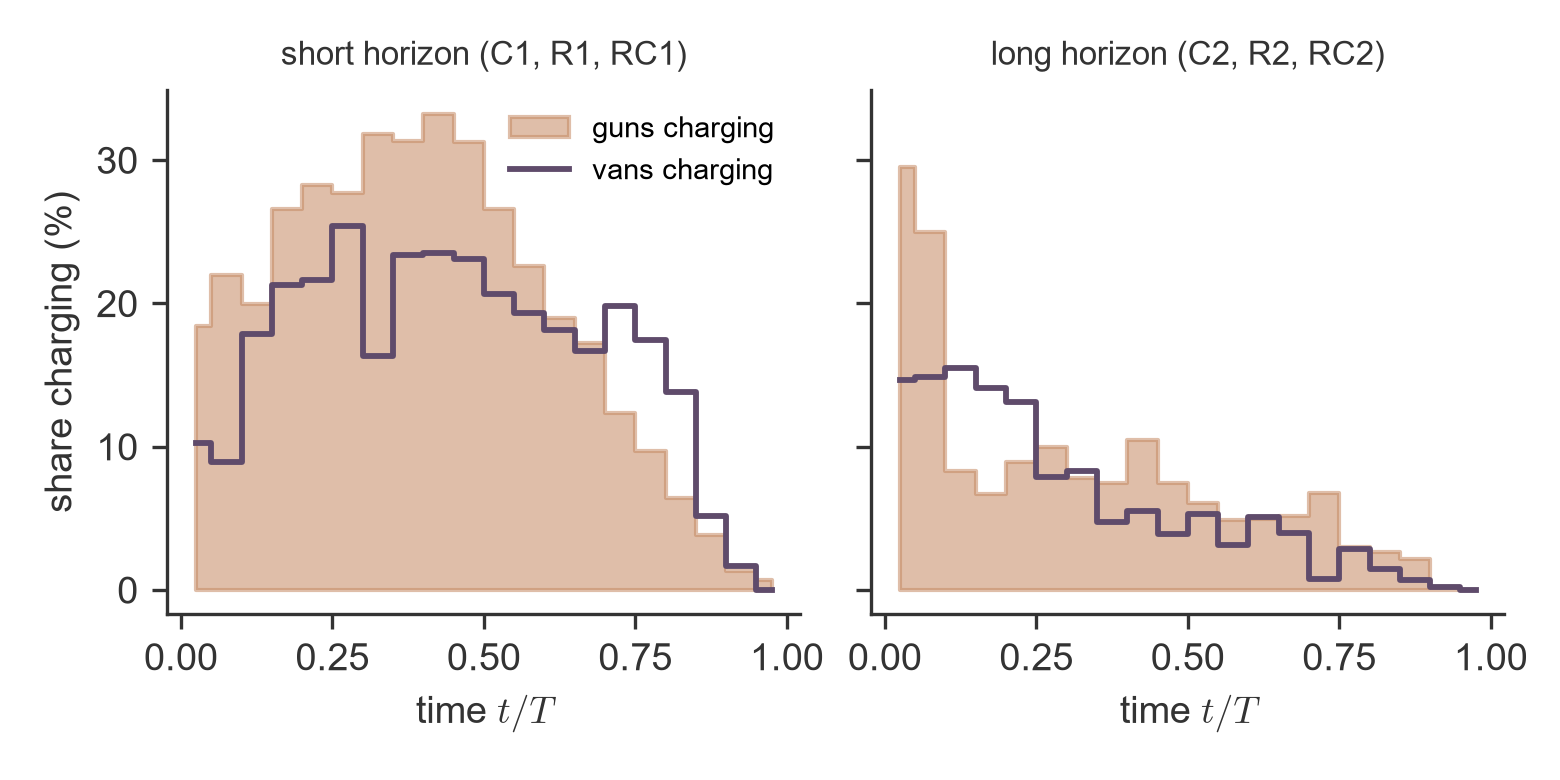
\includegraphics[width=\textwidth]{figures/busy.png}

\scriptsize Share of guns and vans charging over time (MILP).
\column{.42\textwidth}
\small
\begin{itemize}
  \item Guns busy \GunUtilMilp\% (MILP), \GunUtilRl\% (RL); \GunUtilShort\% short, \GunUtilLong\% long horizons.
  \item \GunsNeverM\% of guns never used; busiest gun \GunMaxM\%.
  \item Peak: \PeakGunsM{} guns at once; all 24 in \AllGunsBusyPlans{} plans.
\end{itemize}
\end{columns}
\end{frame}

% ======================================================================= 19 infrastructure: vans
\begin{frame}{Infrastructure: vans}
\begin{columns}[T]
\column{.58\textwidth}
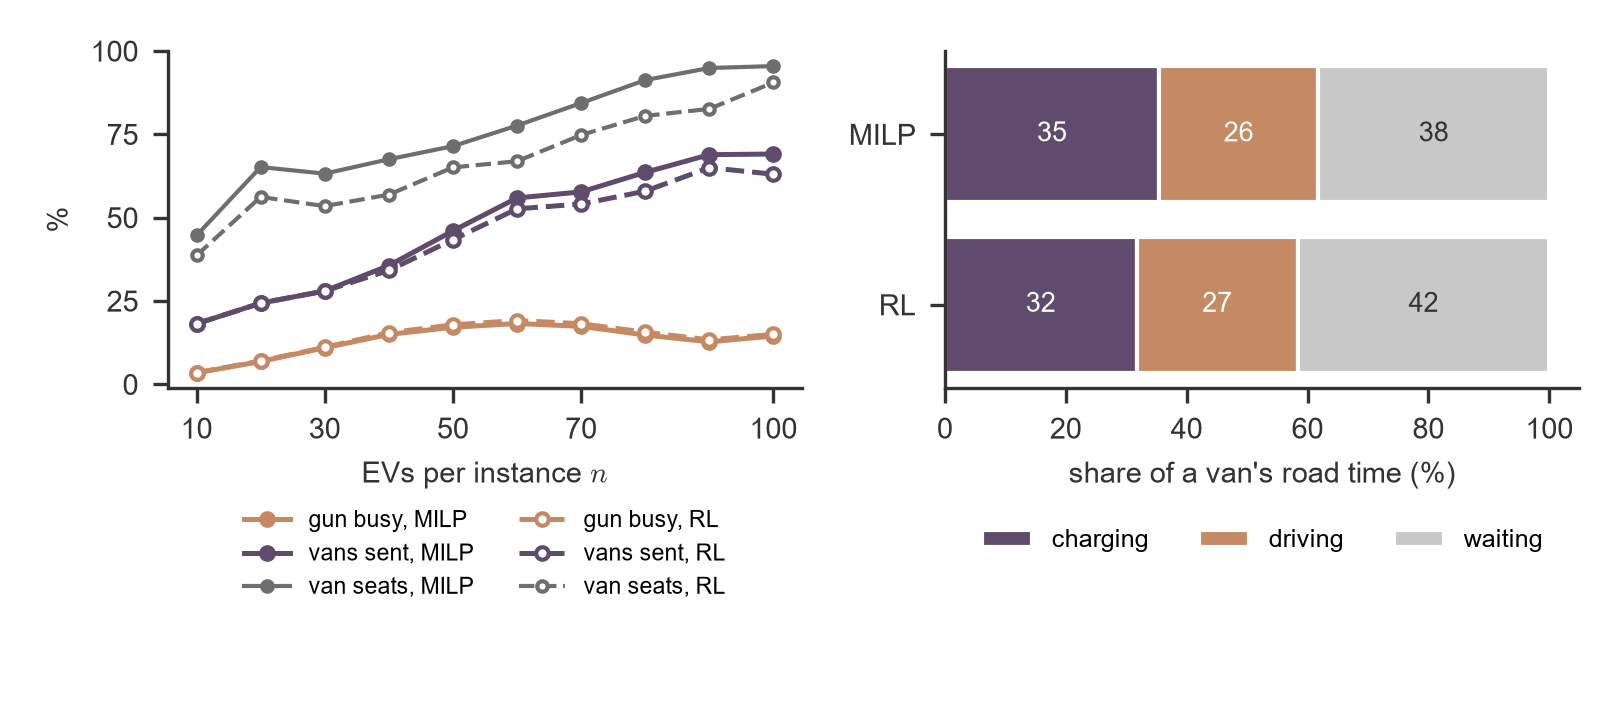
\includegraphics[width=\textwidth]{figures/infra_n.png}
\column{.39\textwidth}
\small
\begin{itemize}
  \item Vans sent \FleetMilp\% (MILP), \FleetRl\% (RL).
  \item Seats \SeatsMilp\% vs \SeatsRl\%; battery \BattMilp\% vs \BattRl\%.
  \item Van energy: \VanDelivShare\% to EVs, \VanLossShare\% loss, \VanDrvEShare\% driving.
  \item RL: fewer, emptier vans.
\end{itemize}
\end{columns}
\end{frame}

% ======================================================================= 20 demand factor: definition
\begin{frame}{Demand factor: definition and levels}
\small
\[
\text{pressure}_i=\frac{\#\{\,j:\ r_i-w\le r_j\le r_i\,\}}{24\text{ guns}+5\text{ vans}},\qquad w=\text{mean station charging time } (\PressWinMin\text{--}\PressWinMax\text{ min})
\]
Low $\le\PressCutLo$ ($\le\PressLoadLo$ requests), high $>\PressCutHi$ ($>\PressLoadHi$); thirds over all 560 instances; data only.

\vspace{.6ex}
\scriptsize
\begin{tabular}{lrrrrrrrrr}
\toprule
 & & \multicolumn{4}{c}{free-choice EVs by van (\%)} & \multicolumn{4}{c}{station queue (min)}\\
 & EVs & \multicolumn{2}{c}{personal} & \multicolumn{2}{c}{taxi} & \multicolumn{2}{c}{personal} & \multicolumn{2}{c}{taxi}\\
pressure & (\%) & MILP & RL & MILP & RL & MILP & RL & MILP & RL\\
\midrule
\TabPress
\bottomrule
\end{tabular}
\end{frame}

% ======================================================================= 21 demand factor: effect
\begin{frame}{Demand factor: what changes}
\begin{columns}[T]
\column{.55\textwidth}
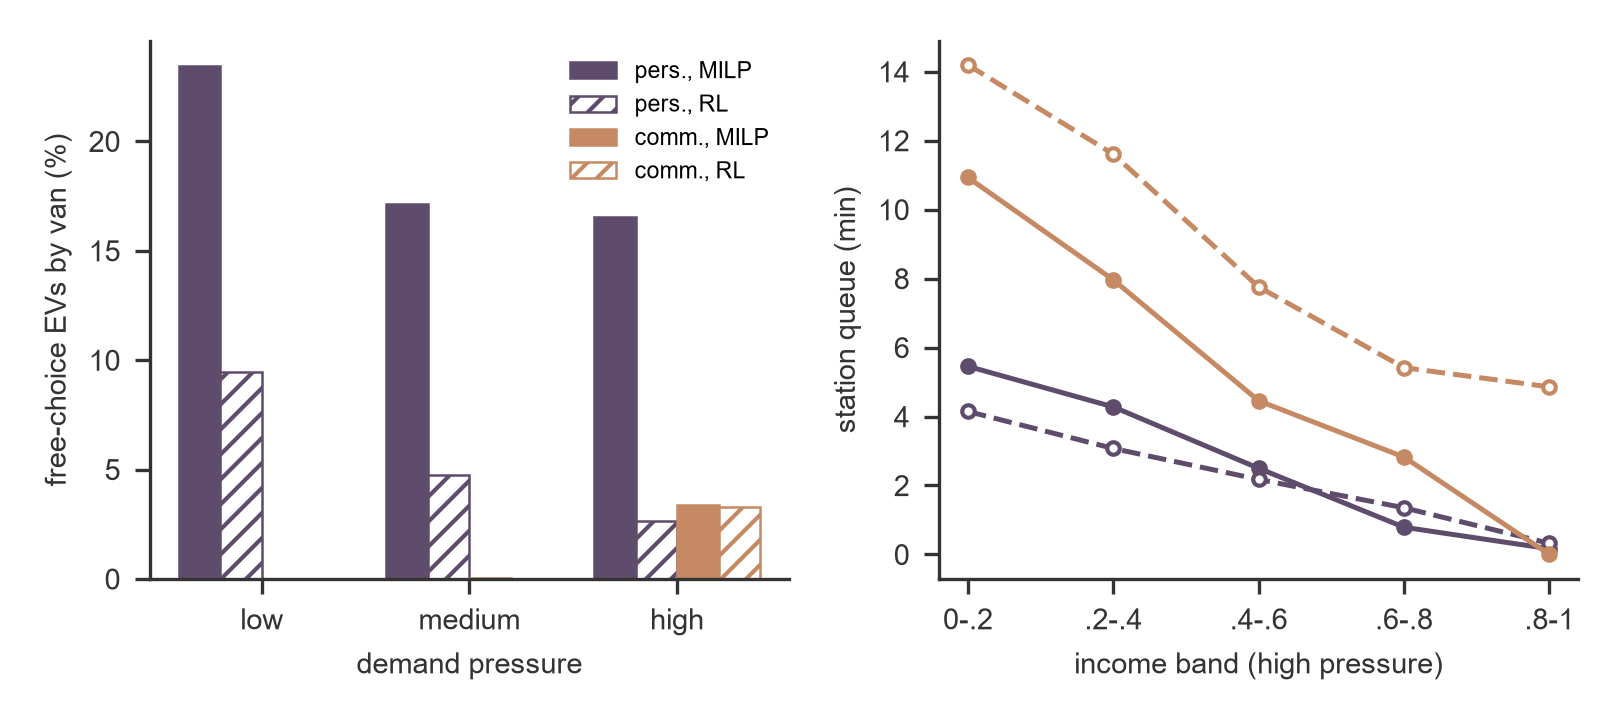
\includegraphics[width=\textwidth]{figures/pressure.png}
\column{.42\textwidth}
\small
\begin{itemize}
  \item Queued: \QueuedLoM\% / \QueuedMedM\% / \QueuedHiM\% (low / medium / high).
  \item Taxis take vans only at high pressure (\VanComHiM\%), poorest first.
  \item Personal vans fall: \VanPersLoM\% $\to$ \VanPersHiM\%.
  \item Higher taxi downtime value does not push taxis to vans at peak (\OmegaHiComHighM{} pts).
\end{itemize}
\end{columns}
\end{frame}

% ======================================================================= 22 experiments
\begin{frame}{Experiments (MILP and RL)}
\begin{columns}[T]
\column{.55\textwidth}
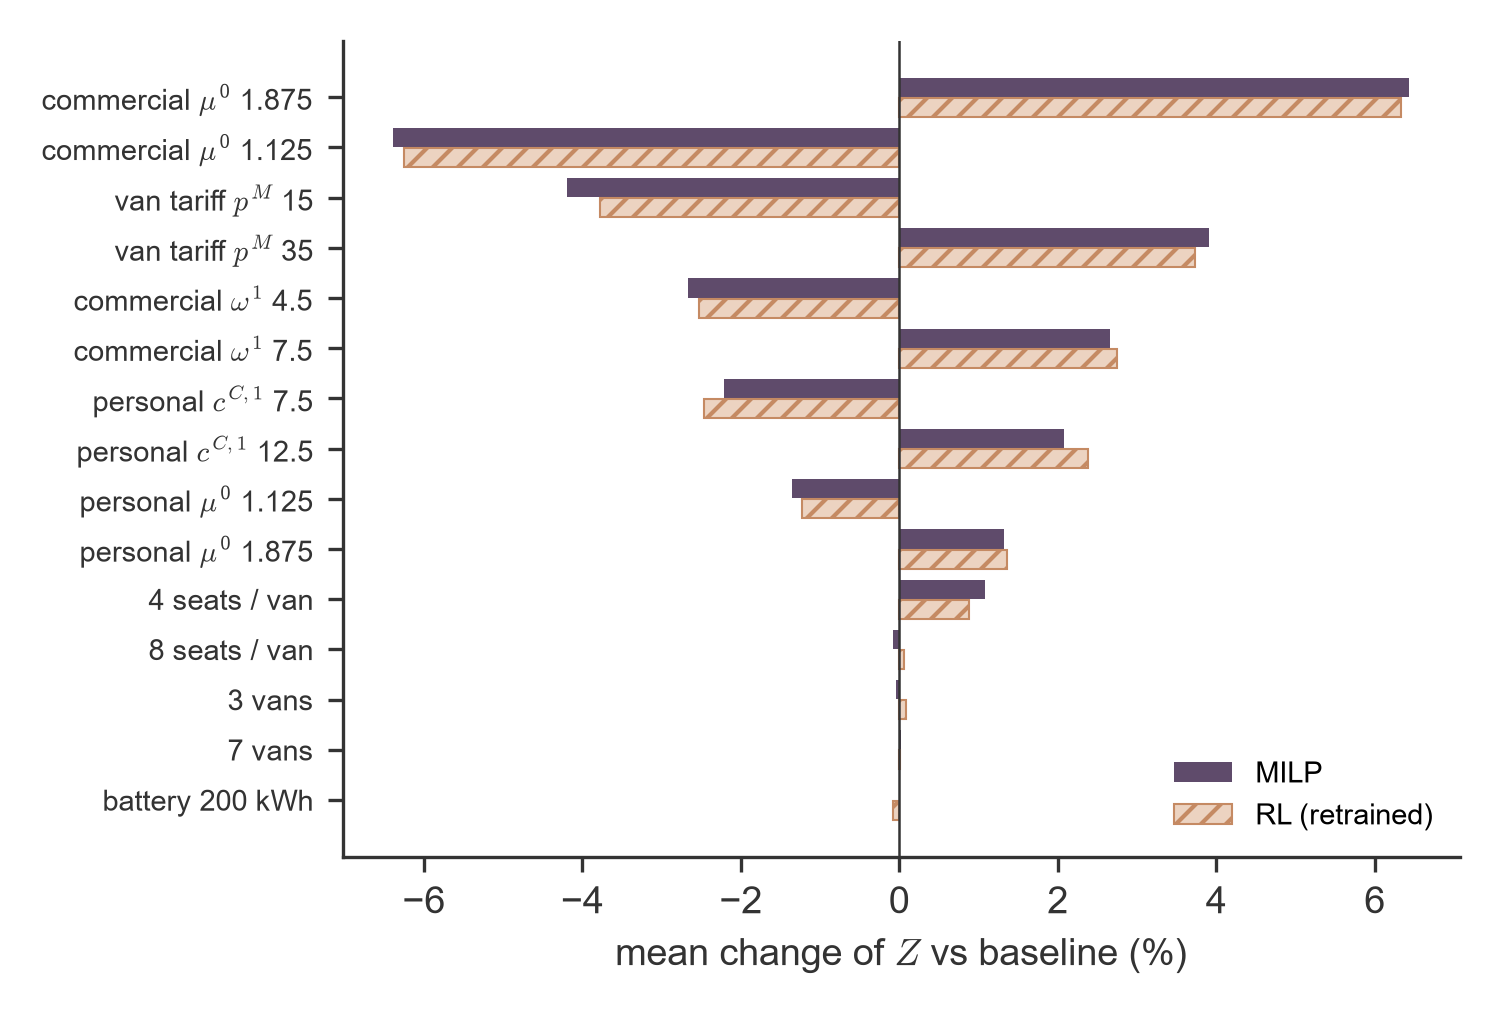
\includegraphics[width=\textwidth]{figures/experiments.png}
\column{.42\textwidth}
\small
\begin{itemize}
  \item Largest: money sensitivity of poor taxis ($Z$ \dZEsixComLo\% / \dZEsixComHi\%).
  \item Van tariff = station price: $Z$ \dZEonePMLo\%, personal vans \dVanEonePMLo{} pts.
  \item 200\,kWh battery: $Z$ \dZEeight\%; recharging can be ignored.
  \item RL follows the MILP's direction.
\end{itemize}
\end{columns}
\end{frame}

% ======================================================================= 23 E9 / E10
\begin{frame}{Station capacity and demand (RL only)}
\begin{columns}[T]
\column{.55\textwidth}
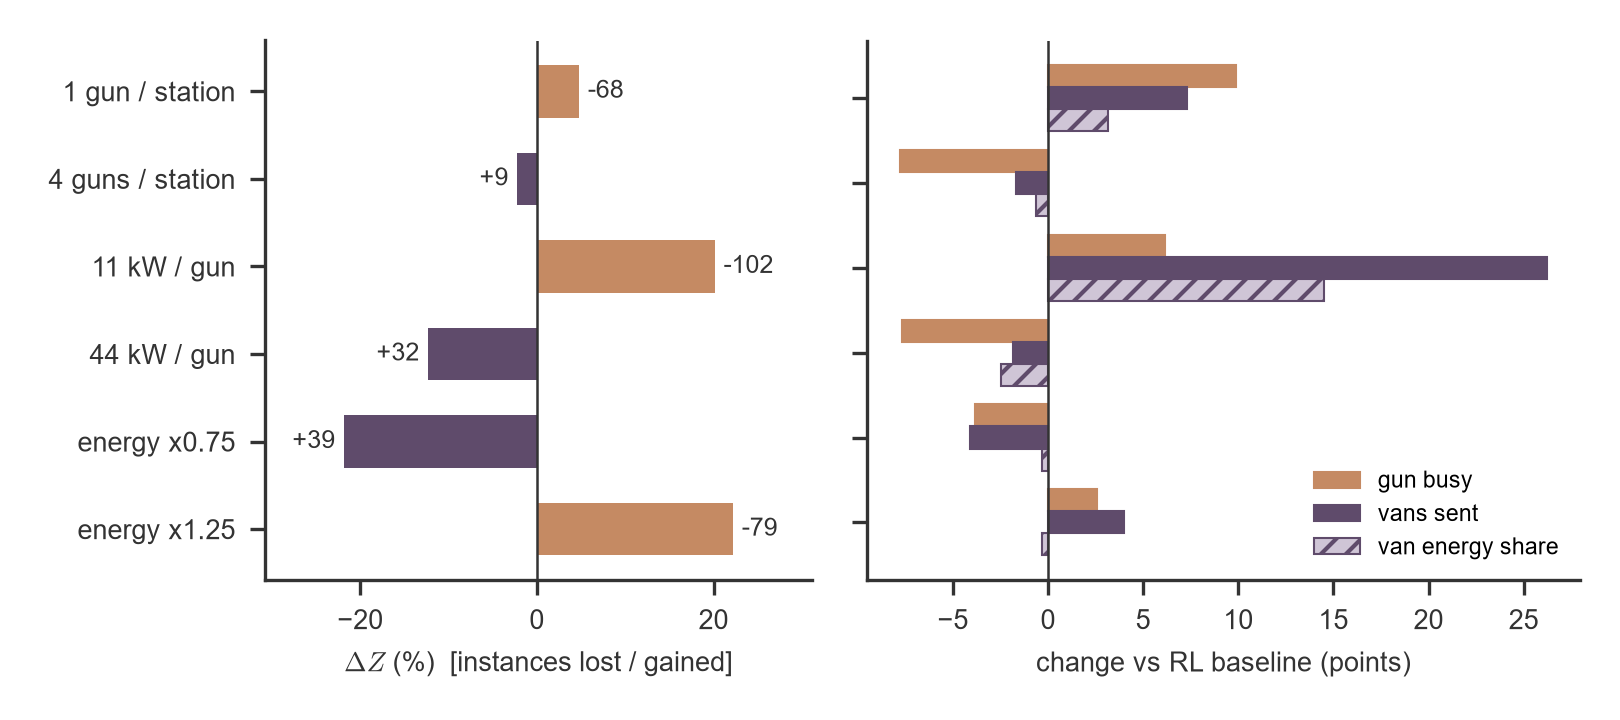
\includegraphics[width=\textwidth]{figures/rl_only.png}
\column{.42\textwidth}
\small
\begin{itemize}
  \item 11\,kW guns: \RLLostPowerEleven{} instances lost, $Z$ \RLdZPowerEleven\%.
  \item 1 gun per station: \RLLostGunsOne{} lost, $Z$ \RLdZGunsOne\%.
  \item 44\,kW guns: \RLNewPowerFortyFour{} gained, $Z$ \RLdZPowerFortyFour\%.
  \item Energy $\pm25\%$: $Z$ \RLdZDemandLow\% / \RLdZDemandHigh\%.
\end{itemize}
\vspace{.5ex}
\scriptsize No MILP run for E9, E10.
\end{columns}
\end{frame}

% ======================================================================= 24 summary
\begin{frame}{Summary}
\begin{itemize}
  \item \textbf{Problem}: assignment and van routing for a charging operator whose customers differ by segment and income.
  \item \textbf{Novelty}: segment- and income-dependent costs in one MILP; an attention policy that picks an EV, then its charger.
  \item \textbf{Benchmarks}: MILP (300\,s) and the greedy rule; RL is \GapMean\% above the MILP, \Speed{}$\times$ faster.
  \item \textbf{Behaviour}: vans go to rich personal owners; taxis do \QShareComM\% of the queueing.
  \item \textbf{RL}: a shared baseline over 8 plans per instance removes the need for a critic.
\end{itemize}
\end{frame}

% ======================================================================= 25 future work
\begin{frame}{Future work}
\begin{itemize}
  \item \textbf{Now}: Monte-Carlo returns of whole plans and policy-gradient updates with a shared baseline.
  \item \textbf{Next in RL}: actor--critic with a learned value baseline; PPO\footnote{J.~Schulman et al., Proximal policy optimization algorithms, arXiv:1707.06347, 2017.} for steadier updates.
  \item \textbf{Model}: calibrate values of time; an evening demand peak; 200-EV instances.
\end{itemize}
\end{frame}

\end{document}
